\setchapterpreamble[u]{\margintoc}
\chapter{Simulating the Glasma}
\labch{simulateglasma}

\begin{preview}[]
The Glasma fields which arise from the collision of two nuclei are described using the previously derived solution for a single nucleus. Initial conditions and equations of motion are derived in the boost-invariant approximation. These are then discretized using principles from real-time lattice gauge theory and then numerically simulated. Details about implementation, numerical parameters, observables are provided, along with results tuned for {\sffamily RHIC} collisions of {\sffamily Au+Au} nuclei at $\sqrt{s_\textsf{NN}}=200$ GeV.  
\end{preview}

\section{Boost-invariant Glasma}

\subsubsection*{Generalized MV model}
In the original {\sffamily MV} model, the small-$x$ partons see the large-$x$ partons as being distributed on an infinitely thin color sheet. The associated color current is thus generated as\sidenote{In comparison with the current from Equation~(\cref{glasma53}).} 
\begin{align}\label{sglasma8}
    J^\mu(x)=\delta^{\mu+}\delta(x^-)\rho(\vec{x}_\perp)
\end{align}
The one-point and two-point functions of the color charge reduce to\sidenote{As opposed to the more general correlators from Equation~(\cref{glasma33a}) and~(\cref{glasma33b}).}
\begin{align*}
&\langle \rho^a\left(\vec{x}_\perp\right)\rangle_A=0,\\
&\langle \rho^a\left(\vec{x}_\perp\right)\rho^b\left(\vec{y}_\perp\right)\rangle_A=\mu^2\delta^{ab}\delta^{(2)}\left(\vec{x}_\perp-\vec{y}_\perp\right),
\end{align*}
where $\mu$ represents the average color charge per unit surface and is usually referred to as the {\sffamily MV} parameter. The transverse pure gauge fields are given by\sidenote{Similarly to Equation~(\cref{glasma16}).} 
\begin{align}\label{sglasma4}
    A^i(x^-,\vec{x}_\perp)=\theta(x^-)\alpha^i(\vec{x}_\perp),
\end{align}
where we introduced the notation
\begin{align}\label{sglasma5}
    \alpha^i(\vec{x}_\perp)\overset{\Delta}{=}\frac{i}{g}\textsf{V}(\vec{x}_\perp)\partial^i\textsf{V}^\dagger(\vec{x}_\perp),
\end{align}
with the asymptotic Wilson line\sidenote{Since it's the more general Wilson line from Equation~(\cref{glasma52}) in the limit $x^-\rightarrow\infty$.}expressed as
\begin{align*}
    \textsf{V}^\dagger(\vec{x}_\perp)&\overset{\Delta}{=}\lim\limits_{x^-\rightarrow\infty}\textsf{W}^\dagger(x^-,\vec{x}_\perp)\\
    &\stackrel{(\text{\cref{glasma52}})}{=\joinrel=\joinrel=}\mathcal{P}\exp{ig\int\limits_{-\infty}^{\infty}dx^-\alpha(x^-,\vec{x}_\perp)}.   
\end{align*}
Here the light-cone gauge solution satisfies a transverse Poisson equation\sidenote{In analogy with Equation~(\cref{glasma20}). The color charge from the covariant gauge may be expressed in terms of the light-cone gauge one as $\widetilde{\rho}=\textsf{V}^\dagger\rho\textsf{V}$, as in Equation~(\cref{glasma21}).}
\begin{align}\label{sglasma3}
    \Delta_\perp\alpha(\vec{x}_\perp)=-\widetilde{\rho}(\vec{x}_\perp).
\end{align}

Nevertheless, for very small-$x$ values, it is more appropriate to consider a color charge with finite longitudinal support\sidenote{For this reason, all the computations from \refch{glasma} were performed in this framework.}$\rho(x^-,\vec{x}_\perp)$, as emphasized in \cite{jalilian}. In this generalized {\sffamily MV} model\sidenote{For which the one-point and two-point correlators are given in Equations~(\cref{glasma33a}) and~(\cref{glasma33b}).}the nucleus may be thought of as being composed of a multitude of uncorrelated infinitely thin sheets of color charge.\sidenote{Because of $\delta(x^--y^-)$ from the two-point correlator given in Equation~(\cref{glasma33b}).}One may not recover the single sheet approximation from the generalized {\sffamily MV} model by simply taking the limit $\rho(x^-,\vec{x}_\perp)\rightarrow\delta(x^-)\rho(\vec{x}_\perp)$. \\
As argued in \cite{fukushima}, one may construct a two-point charge correlator as
\begin{align}\label{sglasma28}
    \langle\rho^a_n(\vec{x}_\perp)\rho^b_m(\vec{y}_\perp)\rangle_A=\mu^2\frac{\delta_{nm}}{N_s}\delta^{ab}\delta^{(2)}(\vec{x}_\perp-\vec{y}_\perp),
\end{align}
where $n,m\in\overline{1,N_s}$ denote the indices of the color sheets and $N_s$ the total number of this stacked sheets of color charge. Each color charge obeys a Poisson equation\sidenote{As in Equation~(\cref{sglasma3}).}
\begin{align}\label{sglasma}
    \Delta_\perp\alpha_n(\vec{x}_\perp)=-\widetilde{\rho}_n(\vec{x}_\perp).
\end{align}
The fields generated by such a color sheet are also given by\sidenote{See Equations~(\cref{sglasma4} and~(\cref{sglasma5}).}
\begin{align*}
   A^i_n(x^-,\vec{x}_\perp)=\frac{i}{g}\theta(x^-)\textsf{V}(\vec{x}_\perp)\partial^i\textsf{V}^\dagger(\vec{x}_\perp),
\end{align*}
with the Wilson line
\begin{align}\label{sglasma30}
    \textsf{V}^\dagger(\vec{x}_\perp)=\prod\limits_{n=1}^{N_s}\exp{ig\alpha_n(\vec{x}_\perp)}.
\end{align}
For $N_s=1$, one obtains the original {\sffamily MV} model, while $N_s\rightarrow\infty$ gives the proper ultrarelativistic limit of the generalized {\sffamily MV} model. As we shall see, $N_s$ will further appear as a numerical parameter.\sidenote{It will influence the relation between the {\sffamily MV} parameter $\mu$ and the saturation momentum $Q_s$.}

\subsubsection*{Constructing the glasma fields} 
The {\sffamily MV} model provides an expression for the classical gauge fields generated by a high-energy nucleus. This analytic solution, which describes the color fields before a collision occurs, may be used to model the melting of the {\sffamily CGC} during the collision of ultrarelativistic nuclei.

\begin{figure}[!hbt]
	\centering
    \includesvg[width=0.7\textwidth]{images/diagrams/regions.svg}
    \caption{\normalsize Light-cone diagram of a collision in the {\sffamily MV} model, where {\sffamily 4} regions distinguish themselves. The Glasma fields produced in the forward light-cone shall further be studied.}
\end{figure}

This may be schematically represented in a light-cone diagram, in which {\sffamily 4} regions emerge. In region {\sffamily 0}, since it is enclosed in the past light-cone and is thus causally disconnected from the others, the gauge field may be set to be null $A^\mu_{\textsf{0}}=0$. In regions {\sffamily 1} and {\sffamily 2}, one may employ the {\sffamily MV} solutions and express the fields as\sidenote{Notice that we write the most general solution, without employing the previously introduced generalization of the {\sffamily MV} model.}
\begin{align}\label{sglasma1}
    A^i_{\textsf{1},\textsf{2}}(x^\mp,\vec{x}_\perp)=\frac{i}{g}\textsf{W}_{\textsf{1},\textsf{2}}(x^\mp,\vec{x}_\perp)\partial^i\textsf{W}_{\textsf{1},\textsf{2}}^\dag(x^\mp,\vec{x}_\perp),
\end{align}
expressed in terms of the Wilson lines
\begin{align*}
    \textsf{W}_{\textsf{1},\textsf{2}}^\dag(x^\mp,\vec{x}_\perp)=\mathcal{P}\exp{-ig\int\limits_{-\infty}^{x^\mp}dz^\mp\frac{1}{\nabla_\perp^2}\widetilde{\rho}_{\textsf{1},\textsf{2}}(z^\mp,\vec{x}_\perp)}.
\end{align*}

\begin{note}
Let us recall that\sidenote{For a nucleus, which we shall label with $\textsf{1}$, moving along the $x^+$ axis, working in the light-cone gauge $A^+_\textsf{1}=0$, with only transverse color fields $A^i_\textsf{1}$ generated by a color charge distribution $\rho_1$.}
\begin{align*}
    A^i_\textsf{1}(x^-,\vec{x}_\perp)\stackrel{(\text{\cref{glasma16}})}{=\joinrel=\joinrel=}\frac{i}{g}\textsf{W}_\textsf{1}(x^-,\vec{x}_\perp)\partial^i\textsf{W}_\textsf{1}^\dag(x^-,\vec{x}_\perp),
\end{align*}
with the Wilson line given by
\begin{align*}
    \textsf{W}_\textsf{1}^\dag(x^-,\vec{x}_\perp)\underset{(\text{\cref{glasma20}})}{\stackrel{(\text{\cref{glasma52}})}{=\joinrel=\joinrel=}}\mathcal{P}\exp{-ig\int\limits_{-\infty}^{x^-}dz^-\frac{1}{\nabla_\perp^2}\widetilde{\rho}_\textsf{1}(z^-,\vec{x}_\perp)}.
\end{align*}
In a similar manner, one may write the fields produced by the other nucleus\sidenote{By inverting $x^+\leftrightarrow x^-$, for nucleus $\textsf{2}$ moving along the $x^-$ axis, working in the light-cone gauge $A^-_\textsf{2}=0$, with only transverse color fields $A^i_\textsf{2}$ generated by a color charge distribution $\rho_\textsf{2}$.}
\begin{align*}
    A^i_\textsf{2}(x^+,\vec{x}_\perp)=\frac{i}{g}\textsf{W}_\textsf{2}(x^+,\vec{x}_\perp)\partial^i\textsf{W}_\textsf{2}^\dag(x^+,\vec{x}_\perp),
\end{align*}
with the Wilson line given by
\begin{align*}
    \textsf{W}_\textsf{2}^\dag(x^+,\vec{x}_\perp)=\mathcal{P}\exp{-ig\int\limits_{-\infty}^{x^+}dz^+\frac{1}{\nabla_\perp^2}\widetilde{\rho}_\textsf{2}(z^+,\vec{x}_\perp)}.
\end{align*}
\end{note}

These fields generated from region {\sffamily 3} are conventionally named the {\sffamily\color{ming}Glasma} color fields. They are generated by the total color current
\begin{align*}
    J^\mu_\textsf{3}(x)&=J^\mu_\textsf{1}(x)+J^\mu_\textsf{2}(x)\\
    &\stackrel{(\text{\cref{glasma53}})}{=\joinrel=\joinrel=}\delta^{\mu+}\rho_\textsf{1}(x^-,\vec{x}_\perp)+\delta^{\mu-}\rho_\textsf{2}(x^+,\vec{x}_\perp).
\end{align*}
As we shall see, the Glasma fields may be written in terms of the single-nucleus solutions,\sidenote{From Equation~(\cref{sglasma1}).}with the appropriate boundary conditions and equations of motion. \\
We may further employ the infinitely thin sheet approximation\sidenote{See Equation~(\cref{sglasma4}).}and express the fields as\sidenote{With $\alpha^i_{\textsf{1},\textsf{2}}(\vec{x}_\perp)$ obeying Equation~(\cref{glasma5}).} 
\begin{align*}
    A^i_{\textsf{1},\textsf{2}}(x^\mp,\vec{x}_\perp)=\theta(x^\mp)\alpha^i_{\textsf{1},\textsf{2}}(\vec{x}_\perp).
\end{align*}
Before the collision, the fields from regions {\sffamily 0}, {\sffamily 1} and {\sffamily 3} may be written in a compact manner, by stitching together the fields generated by the two nuclei, as 
\begin{fullwidth}
\begin{equation}\label{sglasma6}
\begin{aligned}
    &A^{\pm}_{\textsf{0},\textsf{1},\textsf{2}}(x)=0,\\
    &A^i_{\textsf{0},\textsf{1},\textsf{2}}(x)=\theta(-x^+)\theta(x^-)\alpha^i_\textsf{1}(\vec{x_\perp})+\theta(x^+)\theta(-x^-)\alpha^i_\textsf{2}(\vec{x_\perp}).
\end{aligned}    
\end{equation}
\end{fullwidth}

In regions {\sffamily 1} and {\sffamily 2}, one imposes the light-cone gauge fixing $A^+_\textsf{1}=A^-_\textsf{2}=0$. Recall that, in order for the light-cone current to be covariantly conserved,\sidenote{And not to experience a color rotation.}one must also choose\sidenote{See Equation~(\cref{glasma12})} $A^-_{\textsf{1}}=0$, and analogously $A^+_{\textsf{2}}=0$. These relations should remain valid at the boundary between region {\sffamily 3} and regions {\sffamily 1} and {\sffamily 2}. For this reason, in region {\sffamily 3} it is appropriate to use the Fock-Schwinger gauge\sidenote{Notice that this choice assures vanishing $A^-_{\textsf{1}}=A^+_\textsf{2}=0$ along the $x^\pm$ axis of the light-cone current.}
\begin{align*}
    x^+A^-_\textsf{3}+x^-A^+_\textsf{3}=0.
\end{align*}

After the collision, the fields from region {\sffamily 3} may be chosen as\sidenote{In order to satisfy the Fock-Schwinger gauge condition.}
\begin{equation}\label{sglasma7}
\begin{aligned}
    &A^+_\textsf{3}(x)=x^+\alpha^\eta(x),\\
    &A^-_\textsf{3}(x)=-x^-\alpha^\eta(x),\\
    &A^i_\textsf{3}(x)=\alpha^i(x).
\end{aligned}    
\end{equation}

A general solution may be constructed by patching together the proposed solutions from all the regions\sidenote{By using Equations~(\cref{sglasma6}) and~(\cref{sglasma7}).}
\begin{fullwidth}
\begin{subequations}
\begin{align}
    &A^+(x)=\theta(x^+)\theta(x^-)x^+\alpha^\eta(x),\label{sglasma9a}\\
    &A^-(x)=-\theta(x^+)\theta(x^-)x^-\alpha^\eta(x),\label{sglasma9b}\\
    &A^i(x)=\theta(x^+)\theta(x^-)\alpha^i(x)+\theta(-x^+)\theta(x^-)\alpha^i_\textsf{1}(\vec{x_\perp})+\theta(x^+)\theta(-x^-)\alpha^i_\textsf{2}(\vec{x_\perp}).\label{sglasma9c}
\end{align}
\end{subequations}
\end{fullwidth}


\subsubsection*{Boost-invariant fields} 
In the original {\sffamily MV} model for the color current generated by a nucleus is given by\sidenote{See Equation~(\cref{sglasma8}).}
\begin{align}\label{sglasma29}
    J^\mu_{\textsf{1},\textsf{2}}(x)=\delta^{\mu\pm}\delta(x^\mp)\rho_{\textsf{1},\textsf{2}}(\vec{x}_\perp),
\end{align}
which then yields a total color current
\begin{align*}
    J^\mu_\textsf{3}(x)=\delta^{\mu+}\delta(x^-)\rho_\textsf{1}(\vec{x}_\perp)+\delta^{\mu-}\delta(x^+)\rho_\textsf{2}(\vec{x}_\perp).
\end{align*}
Such a current is boost invariant, symmetry which will then be passed on to the fields generated by it. 

\begin{note}
By applying a longitudinal Lorentz boost,\sidenote{With velocity $v$.}the light-cone coordinates transform as\sidenote{Where we introduce the rapidity
\begin{align*}
    \beta=\frac{1}{2}\ln{\frac{1+v}{1-v}}.
\end{align*}
}
\begin{align*}
    x^\pm\mapsto x^{\prime\pm}=\mathrm{e}^{\pm\beta}x^\pm, \quad \vec{x}_\perp\mapsto \vec{x}_\perp^\prime=\vec{x}_\perp.
\end{align*}
Hence, the only non-vanishing component of the color current\sidenote{More precisely, $J_\textsf{1}^+$ for nucleus {\sffamily 1} and $J_\textsf{2}^-$ for nucleus {\sffamily 2}.}becomes
\begin{align*}
    J^\pm(x)\mapsto J^{\pm\prime}(x)=\mathrm{e}^{\pm\beta}J^\pm(x),
\end{align*}
which for the {\sffamily MV} model remains unchanged by this Lorentz boost
\begin{fullwidth}
\begin{align*}
    J_{\textsf{1},\textsf{2}}^\pm(x)\mapsto \mathrm{e}^{\pm\beta}\delta(x^\mp)\rho_{\textsf{1},\textsf{2}}(\vec{x}_\perp)=\underbrace{\mathrm{e}^{\pm\beta}\delta(\mathrm{e}^{\pm\beta}x^{\prime\mp})}_{\textstyle\delta(x^{\prime\mp})}\rho_{\textsf{1},\textsf{2}}(\vec{x}^\prime_\perp)=J_{\textsf{1},\textsf{2}}^\pm(x^\prime).
\end{align*}
\end{fullwidth}
\end{note}

For this reason, in region {\sffamily 3} we shall use a special set of coordinates\sidenote{In which the condition of boost-invariance of the fields suppresses any $\eta$ dependence 
\begin{align*}
    &\alpha^\eta(x)=\alpha^\eta(\tau,\vec{x}_\perp),\\
    &\alpha^i(x)=\alpha^i(\tau,\vec{x}_\perp).
\end{align*}
}$(x^+,\vec{x}_\perp,x^-)\mapsto (\tau,\vec{x}_\perp,\eta)$, where the proper time $\tau$ and space-time rapidity $\eta$ are defined as
\begin{subequations}
\coloredeqnums{
&\tau\overset{\Delta}{=}\sqrt{2x^+x^-},\label{sglasma12a}\\
&\eta\overset{\Delta}{=}\frac{1}{2}\ln{\left(\frac{x^+}{x^-}\right)}.\label{sglasma12b}
}
\end{subequations}

\begin{marginfigure}[-5.5cm]
	\centering
    \includesvg[width=\textwidth]{images/diagrams/etatau.svg}
    \caption*{Diagram of light-cone and boost-invariant coordinates.}
\end{marginfigure}


The gauge fields transform accordingly, yielding a null temporal component\sidenote{For this reason, the Fock-Schwinger gauge is also called the temporal gauge.}
\begin{align*}
    A^\tau=\frac{1}{\tau}\cancelto{0}{\big(x^-A^++x^+A^-\big)}=0,
\end{align*}
and similarly
\begin{align*}
    A^\eta(x)&=\frac{1}{\tau^2}\big(x^-A^+-x^+A^-\big)\\
    &\underset{(\text{\cref{sglasma9b}})}{\stackrel{(\text{\cref{sglasma9a}})}{=\joinrel=\joinrel=\joinrel=}}\frac{1}{\cancel{2x^-x^+}}\theta(x^+)\theta(x^-)\cancel{2x^-x^+}\alpha^\eta(\tau,\vec{x}_\perp).
\end{align*}

\begin{note}
Simple manipulations lead to the useful relations
\begin{fullwidth}
\begin{align}\label{sglasma10}
    \frac{\partial\tau}{\partial x^\pm}\stackrel{(\text{\cref{sglasma12a}})}{=\joinrel=\joinrel=\joinrel=}\frac{\partial}{\partial x^\pm}(\sqrt{2x^+x^-})=\frac{x^\pm}{\sqrt{2x^+x^-}}\stackrel{(\text{\cref{sglasma12a}})}{=\joinrel=\joinrel=\joinrel=}\frac{x^\pm}{\tau}
\end{align}
\end{fullwidth}
and analogously
\begin{fullwidth}
\begin{align}\label{sglasma11}
    \frac{\partial\eta}{\partial x^\pm}\stackrel{(\text{\cref{sglasma12b}})}{=\joinrel=\joinrel=\joinrel=}\frac{\partial}{\partial x^\pm}\left[\frac{1}{2}\ln\left(\frac{x^+}{x^-}\right)\right]=\pm\frac{1}{2x^\pm}\stackrel{(\text{\cref{sglasma12a}})}{=\joinrel=\joinrel=\joinrel=}\pm\frac{x^\mp}{\tau}.
\end{align}
\end{fullwidth}
The gauge fields may be expressed in the coordinates $(\tau,\eta)$ by applying a transformation
\begin{align*}
    A^\mu(x^\prime)=\frac{\partial x^{\prime\mu}}{\partial x^\nu}A^\nu(x),
\end{align*}
which for $\mu=\tau$ yield
\begin{align*}
    A^\tau=\frac{\partial\tau}{\partial x^+}A^++\frac{\partial\tau}{\partial x^-}A^-\stackrel{(\text{\cref{sglasma10}})}{=\joinrel=\joinrel=}\frac{1}{\tau}(x^-A^++x^+A^-)
\end{align*}
and for $\mu=\eta$ give
\begin{align*}
    A^\eta=\frac{\partial\eta}{\partial x^+}A^++\frac{\partial\eta}{\partial x^-}A^-\stackrel{(\text{\cref{sglasma11}})}{=\joinrel=\joinrel=}\frac{1}{\tau^2}(x^-A^+-x^+A^-).
\end{align*}
\end{note}

The solution is thus completely given by\sidenote{Together with the result from Equation~(\cref{sglasma9c}).}

\vspace{0.5cm}

\begin{fullwidth}
\coloredeqnum{sglasma24}{
\begin{aligned}
    &A^i(x)=\theta(x^+)\theta(x^-)\alpha^i(\tau,\vec{x}_\perp)+\theta(-x^+)\theta(x^-)\alpha^i_\textsf{1}(\vec{x_\perp})+\theta(x^+)\theta(-x^-)\alpha^i_\textsf{2}(\vec{x_\perp})\\
    &A^\eta(x)=\theta(x^+)\theta(x^-)\alpha^\eta(\tau,\vec{x}_\perp).
\end{aligned}
}
\end{fullwidth}


\subsubsection*{Boost-invariant equations of motion} 
The Yang-Mills action expressed in flat coordinates is given by\sidenote{See the gluon Lagrangian from Equation~(\cref{qcd12})}
\begin{align}\label{sglasma13}
    \textsf{S}=\int\mathrm{d}^4x\left(-\frac{1}{2}\textsf{Tr}\left\{F_{\mu\nu}F^{\mu\nu}\right\}\right),
\end{align}
which in $(\tau,\eta)$ coordinates becomes
\begin{fullwidth}
\begin{align}\label{sglasma14}
    \textsf{S}=\int\mathrm{d}\tau\mathrm{d}^2\vec{x}_\perp\mathrm{d}\eta\textsf{Tr}\left\{\tau F_{\tau i}F_{\tau i}+\frac{1}{\tau}F_{\tau\eta}F_{\tau\eta}-\frac{\tau}{2}F_{ij}F_{ij}-\frac{1}{\tau}F_{\eta i}F_{\eta i}\right\}.
\end{align}
\end{fullwidth}

\begin{note}
The metric tensor in the $(\tau,\eta)$ coordinates becomes\sidenote{And similarly
\begin{align*}
    g^{\mu\nu}=\textsf{Diag}\{1, -1, -1, -1/\tau^2\}.
\end{align*}
}
\begin{align*}
    g_{\mu\nu}=\textsf{Diag}\{1, -1, -1, -\tau^2\}.
\end{align*}
The infinitesimal volume element is given by
\begin{align*}
    \mathrm{d}^4 x=\underbrace{\sqrt{\textsf{Det}\textsf{ g}}}_{\textstyle\tau}\mathrm{d}\tau\mathrm{d}^2\vec{x}_\perp\mathrm{d}\eta.
\end{align*}
Therefore, one may express the Yang-Mills action\sidenote{From Equation~(\cref{sglasma13}).}as
\begin{fullwidth}
\begin{align*}
    \textsf{S}&=-\int\mathrm{d}\tau\mathrm{d}^2\vec{x}_\perp\mathrm{d}\eta\frac{1}{\cancel{2}}\textsf{Tr}\Big\{\cancel{2}\tau F_{\tau i}\underbrace{F^{\tau i}}_{\textstyle-F_{\tau i}}+\cancel{2}\cancel{\tau}F_{\tau\eta}\underbrace{F^{\tau\eta}}_{-\dfrac{F_{\tau\eta}}{\tau^{\cancel{2}}}}+\cancel{2}\frac{\tau}{2}F_{ij}\underbrace{F^{ij}}_{\textstyle F_{ij}}+\cancel{2}\cancel{\tau}F_{\eta i}\underbrace{F^{\eta i}}_{\dfrac{F_{\eta i}}{\tau^{\cancel{2}}}}\Big\}.
\end{align*}
\end{fullwidth}
\end{note}

One may define canonical momenta as
\begin{equation}\label{sglasma16}
\begin{aligned}
    & P^\eta\overset{\Delta}{=}\frac{\delta\textsf{S}}{\delta(\partial_\tau A_\eta)}=\frac{1}{\tau}F_{\tau\eta},\\
    & P^i\overset{\Delta}{=}\frac{\delta\textsf{S}}{\delta(\partial_\tau A_i)}=\tau F_{\tau i}.
\end{aligned}
\end{equation}

Varying this action\sidenote{Given in Equation~(\cref{sglasma14}).} with respect to $A_\tau$, before employing the Fock-Schwinger gauge condition $A_\tau=0$, and requiring that $\delta_\tau\textsf{S}=0$, yields the so-called Gauss constraint
\begin{align}\label{sglasma17}
    \tau\textsf{D}_iF_{\tau i}+\frac{1}{\tau}\textsf{D}_\eta F_{\tau\eta}=0.
\end{align}

\begin{note}
In general, varying the action\sidenote{More concisely
\begin{align*}
    \delta_\mu\textsf{S}\overset{\Delta}{=}\frac{\delta\textsf{S}}{{\color{ming}\delta A_\mu}}.
\end{align*}
}with respect to $A_\mu$ is done through
\begin{equation}\label{sglasma15}
\begin{aligned}
    \delta_\mu F_{\mu\nu}&=\delta_\mu(\partial_\mu A_\nu-\partial_\nu A_\mu +ig[A_\mu,A_\nu])\\
    &=-\partial_\nu{\color{ming}\delta A_\mu}+ig[{\color{ming}\delta A_\mu},A_\nu]=-\textsf{D}_\nu{\color{ming}\delta A_\mu}.
\end{aligned}    
\end{equation}
The only terms from the action which bring contributions\sidenote{For a given $\mu\neq\nu$.}are\sidenote{After performing integration by parts and making use of the trace relation
\begin{align*}
\textsf{Tr}\{\textsf{A}[\textsf{B},\textsf{C}]\}=\textsf{Tr}\{[\textsf{A},\textsf{B}]\textsf{C}\}.  
\end{align*}
Notice that we wrote the most general form, in order to also consider the case for $\mu=\tau$, which has an extra $\tau$ from the volume element and any additional ones that may come from lowering the indices of $F^{\mu\nu}$.
}
\begin{align*}
    \delta_\mu\textsf{S}&=\delta_\mu\Big(\int\mathrm{d}^4x\textsf{Tr}\{F_{\mu\nu}F^{\mu\nu}\}\Big)=\int\mathrm{d}^4x\textsf{Tr}\{\delta_\mu(F_{\mu\nu}F^{\mu\nu})\}\\
    &=2\int\mathrm{d}^4x\textsf{Tr}\{F^{\mu\nu}\delta_\mu F_{\mu\nu}\}\stackrel{(\text{\cref{sglasma15}})}{=\joinrel=\joinrel=}2\int\mathrm{d}^4x\textsf{Tr}\{F^{\mu\nu}(-\textsf{D}_\nu{\color{ming}\delta A_\mu})\}\\
    &=2\Big[\textsf{Tr}\big\{\underbrace{-\int\mathrm{d}\tau\mathrm{d}^2\vec{x}_\perp\mathrm{d}\eta\tau F^{\mu\nu}\partial_\nu{\color{ming}\delta A_\mu}}_{\mathclap{\textstyle\int\mathrm{d}\tau\mathrm{d}^2\vec{x}_\perp\mathrm{d}\eta{\color{ming}\delta A_\mu} \partial_\nu(\tau F^{\mu\nu})+\cancelto{0}{\text{surface term}}}}\big\}+\\
    &\phantom{=}+ig\int\mathrm{d}\tau\mathrm{d}^2\vec{x}_\perp\mathrm{d}\eta\underbrace{\textsf{Tr}\left\{\tau F^{\mu \nu}[{\color{ming}\delta A_\mu},A_\nu]\right\}}_{\textstyle-\textsf{Tr}\left\{[\tau F^{\mu \nu},A_\nu]{\color{ming}\delta A_\mu}\right\}}\Big]\\
    &=2\int\mathrm{d}\tau\mathrm{d}^2\vec{x}_\perp\mathrm{d}\eta\textsf{Tr}\Big\{\underbrace{[\partial_\nu(\tau F^{\mu\nu})+ig[A_\nu,\tau F^{\mu\nu}]]}_{\textstyle\textsf{D}_\nu (\tau F^{\mu\nu})}{\color{ming}\delta A_\mu}\Big\}.
\end{align*}
Summarizing, we obtain
\begin{fullwidth}
\begin{align}\label{sglasma19}
    \delta_\mu\Big(\int\mathrm{d}^4x\textsf{Tr}\big\{F_{\mu\nu}F^{\mu\nu}\}\Big)=2\int\mathrm{d}\tau\mathrm{d}^2\vec{x}_\perp\mathrm{d}\eta\textsf{Tr}\{\textstyle\textsf{D}_\nu (\tau F^{\mu\nu}){\color{ming}\delta A_\mu}\big\}.
\end{align}
\end{fullwidth}


Hence, the variation of the action with respect to $A_\tau$ gives
\begin{align*}
    \delta_\tau\textsf{S}&=\delta_\tau\left(\int\mathrm{d}\tau\mathrm{d}^2\vec{x}_\perp\mathrm{d}\eta\textsf{Tr}\left\{\tau F_{\tau i}F_{\tau i}+\frac{1}{\tau}F_{\tau\eta}F_{\tau\eta}\right\}\right)\\
    &\stackrel{(\text{\cref{sglasma19}})}{=\joinrel=\joinrel=}2\int\mathrm{d}\tau\mathrm{d}^2\vec{x}_\perp\mathrm{d}\eta\textsf{Tr}\left\{\left(\tau\textsf{D}_iF_{\tau i}+\frac{1}{\tau}\textsf{D}_\eta F_{\tau\eta}\right){\color{ming}\delta A_\tau}\right\},
\end{align*}
which after imposing $\delta_\tau\textsf{S}=0$ gives the Gauss constraint.\sidenote{From Equation~(\cref{sglasma17}).}
\end{note}

Therefore, this relation may equivalently be expressed in terms of the momenta as\sidenote{\color{black}Using Equations~(\cref{sglasma16}) and~(\cref{sglasma17}).}
\begin{align}\label{sglasma23}
    \textsf{D}_i P^i+\textsf{D}_\eta P^\eta=0.
\end{align}
Nevertheless, in the temporal gauge $A_\tau=0$ and boost-invariant scenario\sidenote{All the fields $A_\mu$ with $\mu=\tau, i$ are independent of $\eta$.}$\partial_\eta A_\mu=0$, the action simplifies to

\vspace{0.5cm}

\begin{fullwidth}
\coloredeqnum{sglasma18}{
    \textsf{S}=\int\mathrm{d}\tau\mathrm{d}^2\vec{x}_\perp\mathrm{d}\eta\textsf{Tr}\left\{\tau\partial_\tau A_i\partial_\tau A_i +\frac{1}{\tau}\partial_\tau A_\eta\partial_\tau A_\eta-\frac{\tau}{2}F_{ij}F_{ij}-\frac{1}{\tau}\textsf{D}_iA_\eta\textsf{D}_iA_\eta\right\}.
}
\end{fullwidth}

\begin{note}
This may easily be proven by noticing that\sidenote{With $\mu=i,\eta$.}
\begin{align}\label{sglasma20}
    F_{\tau \mu}=\partial_\tau A_\mu-\partial_\mu\cancelto{0}{A_\tau}-ig[A_\mu,\cancelto{0}{A_\tau}],
\end{align}
and similarly
\begin{align}\label{sglasma21}
    F_{\eta i}=\cancelto{0}{\partial_\eta A_i}-\partial_iA_\eta-ig[A_\eta,A_i]=-\textsf{D}_iA_\eta.
\end{align}
Plugging these results back in the action in $(\tau,\eta)$ coordinates\sidenote{From Equation~(\cref{sglasma14}).}immediately leads to the boost-invariant action.\sidenote{See Equation~(\cref{sglasma18}).}
\end{note}

Within this boost-invariant approximation, the Gauss constraint\sidenote{Written in terms of conjugate momenta in Equation~(\cref{sglasma23}).}reduces to
\begin{align}\label{sglasma25}
    \textsf{D}_i P^i+\cancelto{0}{\partial_\eta P^\eta}+ig[A_\eta, P^\eta]=0.
\end{align}

The conjugate momenta further simplify to\sidenote{After inserting the field strengths from Equations~(\cref{sglasma20}) and~(\cref{sglasma21}) back in Equation~(\cref{sglasma16}).}
\begin{subequations}
\begin{align}
    & P^\eta=\frac{1}{\tau}\partial_\tau A_\eta,\label{sglasma22a}\\
    & P^i=\tau\partial_\tau A_i.\label{sglasma22b}
\end{align}
\end{subequations}

Varying this boost-invariant action with respect to the remaining gauge fields, namely $A_\eta$ and $A_i$, provide us with the equations of motion
\begin{equation}\label{sglasma26}
\begin{aligned}
    &\partial_\tau P^i=\tau\textsf{D}_jF_{ji}-\frac{ig}{\tau}[A_\eta,\textsf{D}_iA_\eta],\\
    &\partial_\tau P^\eta=\frac{1}{\tau}\textsf{D}_i(\textsf{D}_iA_\eta).
\end{aligned}    
\end{equation}

\begin{note}
By varying the Yang-Mills action in $(\tau,\eta)$ coordinates\sidenote{From Equation~(\cref{sglasma14}).}with respect to $A_i$ gives
\begin{fullwidth}
\begin{align*}
\delta_i\textsf{S}&=\delta_i\left(\int\mathrm{d}\tau\mathrm{d}^2\vec{x}_\perp\mathrm{d}\eta\textsf{Tr}\left\{\tau F_{i\tau}F_{i\tau}-\frac{\tau}{2}F_{ij}F_{ij}-\frac{1}{\tau}F_{i\eta }F_{i\eta}\right\}\right)\\
&\stackrel{(\text{\cref{sglasma19}})}{=\joinrel=\joinrel=}2\int\mathrm{d}\tau\mathrm{d}^2\vec{x}_\perp\mathrm{d}\eta\textsf{Tr}\left\{\Big(\textsf{D}_\tau\tau F_{i\tau}-\frac{\tau}{2}\textsf{D}_jF_{ij}-\frac{1}{\tau}\textsf{D}_\eta F_{i\eta}\Big){\color{ming}\delta A_i}\right\}.
\end{align*}
\end{fullwidth}
Nevertheless, in the boost-invariant approximation, the above expression becomes
\begin{fullwidth}
\begin{align*}
    \delta_i\textsf{S}&\underset{(\text{\cref{sglasma21}})}{\stackrel{(\text{\cref{sglasma20}})}{=\joinrel=\joinrel=}}2\int\mathrm{d}\tau\mathrm{d}^2\vec{x}_\perp\mathrm{d}\eta\textsf{Tr}\Big\{\Big[(\partial_\tau-ig\cancelto{0}{A_\tau})\tau(-\partial_\tau A_i)-\frac{\tau}{2}\textsf{D}_j(-F_{ji})-\frac{1}{\tau}\big(\cancelto{0}{\partial_\eta\textsf{D}_iA_\eta}-ig[A_\eta,\textsf{D}_iA_\eta]\big)\Big]{\color{ming}\delta A_i}\Big\}\\
    &\stackrel{(\text{\cref{sglasma22a}})}{=\joinrel=\joinrel=\joinrel=}-2\int\mathrm{d}\tau\mathrm{d}^2\vec{x}_\perp\mathrm{d}\eta\textsf{Tr}\Big\{\Big[\partial_\tau\underbrace{(\tau\partial_\tau A_i)}_{\mathclap{\textstyle  P^i}}-\tau\textsf{D}_jF_{ji}+\frac{ig}{\tau}[A_\eta,\textsf{D}_iA_\eta]\Big]{\color{ming}\delta A_i}\Big\}.
\end{align*}
\end{fullwidth}
In a similar manner, the functional derivative of the Yang-Mills action in terms of $A_\eta$ gives
\begin{align*}
    \partial_\eta\textsf{S}&=\partial_\eta\left(\int\mathrm{d}\tau\mathrm{d}^2\vec{x}_\perp\mathrm{d}\eta\textsf{Tr}\left\{\frac{1}{\tau}F_{\eta\tau}F_{\eta\tau}-\frac{1}{\tau}F_{\eta i}F_{\eta i}\right\}\right)\\
    &\stackrel{(\text{\cref{sglasma19}})}{=\joinrel=\joinrel=}2\int\mathrm{d}\tau\mathrm{d}^2\vec{x}_\perp\mathrm{d}\eta\textsf{Tr}\left\{\Big(\textsf{D}_\tau\frac{1}{\tau}F_{\eta\tau}-\frac{1}{\tau}\textsf{D}_iF_{\eta i}\Big){\color{ming}\delta A_\eta}\right\},
\end{align*}
which in the boost-invariant case further simplifies to
\begin{fullwidth}
\begin{align*}
    \partial_\eta\textsf{S}&\underset{(\text{\cref{sglasma21}})}{\stackrel{(\text{\cref{sglasma20}})}{=\joinrel=\joinrel=}}2\int\mathrm{d}\tau\mathrm{d}^2\vec{x}_\perp\mathrm{d}\eta\textsf{Tr}\Big\{\Big[(\partial_\tau-ig\cancelto{0}{A_\tau})\frac{1}{\tau}(-\partial_\tau A_\eta)-\frac{1}{\tau}\textsf{D}_i(-\textsf{D}_iA_\eta)\Big]{\color{ming}\delta A_\eta}\Big\}\\
    &\stackrel{(\text{\cref{sglasma22b}})}{=\joinrel=\joinrel=\joinrel=}2\int\mathrm{d}\tau\mathrm{d}^2\vec{x}_\perp\mathrm{d}\eta\textsf{Tr}\Big\{\Big[-\partial_\tau\underbrace{\Big(\frac{1}{\tau}\partial_\tau A_\eta\Big)}_{\mathclap{\textstyle  P^\eta}}+\frac{1}{\tau}\textsf{D}_i(\textsf{D}_iA_\eta)\Big]{\color{ming}\delta A_\eta}\Big\}.
\end{align*}
\end{fullwidth}
\end{note}

\subsubsection*{Initial conditions} 
Equivalently, one may write the equations of motion for the unknown fields $\alpha^i(\tau,\vec{x}_\perp)$ and $\alpha^\eta(\tau,\vec{x}_\perp)$ as\sidenote{These equations were originally proposed in \cite{kovner1,kovner2}. One may find a detailed derivation in \cite{mcdonald}, in which, as opposed to deriving the equations of motion directly from an action written in $(\tau,\eta)$ coordinates, one expresses all the components of the field strength tensor and then the Yang-Mills equations in these coordinates.}
\begin{align*}
    &\frac{1}{\tau}\textsf{D}_i\partial_\tau\alpha^i+ig\tau\alpha^\eta\partial_\tau\alpha^\eta=0,\\
    &\frac{1}{\tau}\partial_\tau\tau\partial_\tau\alpha^i-ig\tau^2\alpha^\eta\textsf{D}_i\alpha^\eta-\textsf{D}_jF_{ji}=0,\\
    &\frac{1}{\tau^2}\partial_\tau\tau^2\partial_\tau\alpha^\eta-\textsf{D}_i(\textsf{D}_i\alpha^\eta)=0.
\end{align*}
These boost-invariant Yang-Mills equations must be accompanied by initial conditions\sidenote{By inserting the ansatz from Equation~(\cref{sglasma24}) back in the Yang-Mills equations from Equation~(\cref{glasma13}). The presence of the Heaviside functions will give rise, upon repeatedly applying derivatives, to Delta functions. By imposing that their coefficients vanish at $\tau=0$, one obtains initial conditions for $\alpha^i$ and $\alpha^\eta$.}at $\tau\rightarrow 0$
\begin{subequations}
\coloredeqnums{
    &\alpha^i(\tau,\vec{x}_\perp)\Big|_{\tau=0}=\alpha_\textsf{1}^i(\vec{x}_\perp)+\alpha_\textsf{2}^i(\vec{x}_\perp),\label{sglasma27a}\\
    &\alpha^\eta(\tau,\vec{x}_\perp)\Big|_{\tau=0}=\dfrac{ig}{2}[\alpha_\textsf{1}^i(\vec{x}_\perp),\alpha_\textsf{2}^i(\vec{x}_\perp)],\label{sglasma27b}
}
\end{subequations}
along with
\begin{align*}
    \partial_\tau\alpha^i(\tau,\vec{x}_\perp)\Big|_{\tau=0}=\partial_\tau\alpha^\eta(\tau,\vec{x}_\perp)\Big|_{\tau=0}=0.
\end{align*}

\begin{note}
We are going to provide a sketch of this computation, borrowed from \cite{lappistages}, by only looking at the terms\sidenote{Arising from inserting Equation~(\cref{sglasma24}) back in Equation~(\cref{glasma13}).}which have $\delta(x^\pm)$ as coefficients and afterwards cancel those terms. From the Yang-Mills equation for $\mu=i$ one obtains\sidenote{That is $\textsf{D}_\mu F^{\mu i}=0$, a term with $\delta(x^-)\delta(x^+)$ may arise from $\partial_-\partial_+A^i$.}:
\begin{align*}
    \text{coefficient of }\delta(x^-)\delta(x^+):\quad \alpha^i(\tau,\vec{x}_\perp)-\alpha_\textsf{1}^i(\vec{x}_\perp)-\alpha_\textsf{2}^i(\vec{x}_\perp),
\end{align*}
which after integration over the $x^\pm$ components lead to the initial condition\sidenote{See Equation~(\cref{sglasma27a}).}for $\alpha^i$. In a similar manner, the Yang-Mills equation for $\mu=+$ gives\sidenote{That is $\textsf{D}_\mu F^{\mu +}=J^+$ give several contributions through the terms $\partial_-F^{-+}$ and $\textsf{D}_i(-\partial_-A^i)$. The latter one contains
\begin{align*}
    -\partial_-\partial_iA^i=\underbrace{-\delta(x^-)\partial_i\alpha^i_\textsf{1}}_{\mathclap{\textstyle J^+_\textsf{1}}}\theta(x^+).
\end{align*}
}
\begin{align*}
    \text{coefficient of }\delta(x^-)\theta(x^+):\quad 2\alpha^\eta(\tau,\vec{x}_\perp)-ig[\alpha_\textsf{1}^i(\vec{x}_\perp),\alpha_\textsf{2}^i(\vec{x}_\perp)].
\end{align*}
\end{note}

The initial conditions may also be expressed in terms of
\begin{fullwidth}
\begin{equation*}
    \begin{aligned}
        &A_i(\tau,\vec{x}_\perp)\Big|_{\tau=0}=-\alpha^i(\tau,\vec{x}_\perp)\Big|_{\tau=0}, && P^i(\tau,\vec{x}_\perp)\Big|_{\tau=0}=0,\\
        &A_\eta(\tau,\vec{x}_\perp)\Big|_{\tau=0}=0, && P^\eta(\tau,\vec{x}_\perp)\Big|_{\tau=0}=-2\alpha^\eta(\tau,\vec{x}_\perp)\Big|_{\tau=0}.
    \end{aligned}
\end{equation*}
\end{fullwidth}

Provided with initial values and evolution equations,\sidenote{From Equation~(\cref{sglasma26}) with the additional Gauss constraint from Equation~(\cref{sglasma25}) which must be fulfilled at all proper times.}one may discretize them on a lattice and solve them numerically.


\section{Lattice gauge theory}
\subsubsection*{Gauge invariance} 
Nevertheless, a naive discretization of the Yang-Mills action\sidenote{From Equation~(\cref{sglasma13}).}in which one replaces all the partial derivatives\sidenote{Which appear in the field strengths $F^{\mu\nu}$.}with finite differences leads to the loss of gauge invariance \cite{schwartz, peskin}. 

\begin{note}
This is a consequence of imposing local gauge symmetry\sidenote{With a $\textsf{SU}(3)$ gauge transformation given by Equation~(\cref{qcd13}).}of the fields
\begin{align*}
    \phi(x)\mapsto \textsf{U}(x)\phi(x).
\end{align*}
Fields at different space-time points cannot directly be compared.\sidenote{Because of this, the partial derivative, which contains the difference between fields at different points, is not well defined.}By introducing a quantity which gauge transform as
\begin{align}\label{latt3}
    \textsf{W}(x,y)\mapsto\textsf{U}(x)\textsf{W}(x,y)\textsf{U}^\dagger(y),
\end{align}
one may now properly define the covariant derivative as\sidenote{Notice that with this definition, the covariant derivative transforms as
\begin{align}\label{latt1}
    \textsf{D}_\mu\phi(x)\mapsto\textsf{U}(x)\textsf{D}_\mu\phi(x).
\end{align}
}
\begin{align}\label{latt2}
    \textsf{D}_{\mu} \phi(x)\overset{\Delta}{=} \lim _{\delta \epsilon^{\mu} \rightarrow 0} \frac{\textsf{W}(x, x+\epsilon) \phi(x+\epsilon)-\phi(x)}{\epsilon^\mu}.
\end{align}
We choose $\textsf{W}(x,x)=\mathds{1}$ and then write an expansion in terms of the gauge fields\sidenote{If we plug in this relation back in Equation~(\cref{latt2}) and then in Equation~(\cref{latt1}), we deduce the gauge transformation of the gauge fields from Equation~(\cref{qcd10}).}
\begin{align*}
    \textsf{W}(x,x+\epsilon)=1+ig\epsilon^\mu A_\mu+\mathcal{O}(\epsilon^2).
\end{align*}
\end{note}

This enables us to express the {\sffamily\color{ming}Wilson line} as\sidenote{Where the fields may further be written as $A_{\mu}=A_{\mu}^aT^a$ in the fundamental representation.}
\coloredeqnum{latt5}{
    \textsf{W}(x,y)=\mathcal{P}\exp{i g \int_{y}^{x} \mathrm{d} z^{\mu} A_{\mu}(z) }.
}

\begin{note}
The {\sffamily\color{ming}path-ordering} operator $\mathcal{P}\{\ldots\}$ is necessary due to the non-Abelian nature of the fields. More clearly, after writing a Taylor expansion, the path-ordering operator acts as
\begin{fullwidth}
\begin{align*}
    \begin{aligned}
    \textsf{W}(x, y)=& 1+i g \int_{0}^{1} \frac{\mathrm{d} z^{\mu}_\lambda}{\mathrm{d} \lambda} A_{\mu}^{a}(z_\lambda^\mu) T^{a} \mathrm{d} \lambda-\frac{1}{2} g^{2} \int_{0}^{1} \mathrm{d} \lambda \int_{0}^{1} \mathrm{d} \tau \frac{\mathrm{d} z^{\mu}_\lambda}{\mathrm{d} \lambda} \frac{\mathrm{d} z^{\nu}_\tau}{\mathrm{d} \tau}\times\\
    & \times A_{\mu}^{a}(z_\lambda^\mu) A_{\nu}^{b}(z_\tau^\nu)\left[T^{a} T^{b} \theta(\lambda-\tau)+T^{b} T^{a} \theta(\tau-\lambda)\right]+\cdots.
\end{aligned}
\end{align*}
\end{fullwidth}
\end{note}

A Wilson line taken along a closed path $\gamma$ is called a {\sffamily\color{ming}Wilson loop} and it's given by
\coloredeqnum{latt4}{
    \textsf{W}_\gamma=\mathcal{P}\exp{i g \oint\limits_{\gamma} \mathrm{d} x^{\mu} A_{\mu}(x)}.
}
It is important to emphasize that the trace of a Wilson loop is gauge invariant\sidenote{This may easily be proven by inserting Equation~(\cref{latt4}) back in Equation~(\cref{latt3}) and using the invariance of the trace under cyclic permutations.}.

\subsubsection*{Real-time lattice gauge theory} 
Let us begin by discretizing the Minkowski space-time on a hypercubic lattice\sidenote{The lattice spacing along direction $\mu$, with the unit vector is $\widehat{e}^\mu$, is $a^\mu$. This enables us to write $\widehat{a}^{\mu}=a^\mu\widehat{e}^\mu$. More concisely, $a^0$ is the time step and $a^i$ denote the spatial lattice spacings.}whose points are given by
\begin{align*}
    \textsf{X}^4=\left\{x \mid x=\sum_{\mu=0}^{3} n_{\mu} \widehat{a}^{\mu}, \quad n_{\mu} \in \mathbb{Z}\right\}.
\end{align*}
A field $\phi(x)$ which resides on the lattice will be denoted\sidenote{With $x\in\textsf{X}^4$.}as $\phi_x$. The gauge transformation $\textsf{U}(x)$ will become, upon discretization, $\textsf{U}_x$. The discretized action and corresponding field equations written in terms of $A_\mu$ will not remain gauge invariant. \\
Nevertheless, a gauge invariant lattice action may be constructed. Instead of using the gauge fields\sidenote{Along with the corresponding conjugate momenta $P_\mu$.}$A_\mu$ as the main degrees of freedom, one may simply seek for a more suitable quantity which is already gauge invariant and preserves gauge invariance upon discretization. An action built from such a quantity will inherently be gauge invariant. The simplest choice is the trace of a Wilson line.\sidenote{As given in Equation~(\cref{latt4}). We already saw that such a construction is gauge invariant.}  \\
A Wilson line taken between two neighbouring lattice points\sidenote{Namely $x$ and $x+\hat{a}^{\mu}$.}is called a {\sffamily\color{ming}gauge link} and it's given by\sidenote{Here $\overline{\mathcal{P}}\{\ldots\}$ denotes the anti-path-ordering. We introduce the notation
\begin{align*}
    \textsf{W}_{x,\mu}\overset{\Delta}{=}\textsf{W}(x,x+\widehat{a}^{\mu})
\end{align*}
and similarly for $A_{x,\mu}$.
}
\begin{align*}
    \textsf{W}_{x, \mu}=\overline{\mathcal{P}} \exp{i g \int\limits_{x}^{x+\widehat{a}^{\mu}} d x^{\mu} A_{x,\mu}}.
\end{align*}
\begin{note}
In a similar manner, we may also introduce a gauge link along the opposite direction, which would yield
\begin{align}\label{latt6}
    W_{x,\mu}^{\dagger}=\textsf{W}_{x+\mu,-\mu}.
\end{align}

\begin{marginfigure}[-5.5cm]
	\centering
    \includesvg[width=\textwidth]{images/diagrams/plaquette_2d.svg}
    \caption*{Diagram of a plaquette.}
\end{marginfigure}

A gauge link transforms as
\begin{align*}
    \textsf{W}_{x, \mu} \rightarrow \textsf{U}_{x} \textsf{W}_{x, \mu} \textsf{U}_{x+\mu}^{\dagger}.
\end{align*}
One may express a gauge link and afterwards expand it as\sidenote{See Equation~(\cref{latt5}).}
\begin{fullwidth}
\begin{equation}
    \begin{aligned}\label{latt7}
     \textsf{W}_{x,\mu}&=\exp{iga^\mu A_{x,\mu}}\approx \mathds{1}+iga^\mu A_{x,\mu(x)}-\frac{1}{2}g^2a^\mu a^\nu A_{x,\mu}A_
     {x,\nu}+\mathcal{O}(a^3).
\end{aligned}
\end{equation}
\end{fullwidth}

\end{note}
The simplest non-trivial\sidenote{The shortest Wilson line would just go back and forth between two neighbouring sites but such a combination would simply yield the trivial result
\begin{align*}
    \textsf{W}_{x,\mu}\textsf{W}_{x+\mu,-\mu}\stackrel{(\text{\cref{latt6}})}{=\joinrel=\joinrel=}\mathds{1}.
\end{align*}
}Wilson loop on the lattice may be constructed along the path connecting neighbouring points on a rectangular {\sffamily\color{ming}plaquette} as
\begin{align*}
    \textsf{W}_{x, \mu \nu}&=\textsf{W}_{x, \mu} \textsf{W}_{x+\mu, \nu} \textsf{W}^\dagger_{x+\mu,\mu}\textsf{W}^\dagger_{x,\nu}\\
    &\stackrel{(\text{\cref{latt6}})}{=\joinrel=\joinrel=}\textsf{W}_{x, \mu} \textsf{W}_{x+\mu, \nu} \textsf{W}_{x+\mu+\nu,-\mu} \textsf{W}_{x+\nu,-\nu},
\end{align*}
which may further be expressed as
\begin{align*}
    \textsf{W}_{x, \mu \nu} \approx \exp{ig a^{\mu} a^{\nu} F_{x,\mu \nu}+\mathcal{O}\left(a^{3}\right)}.
\end{align*}

\begin{note}
We may write the discretized Wilson loop as\sidenote{
Using the Campbell-Baker-Hausdorff formula
\begin{align*}
    &\exp{\textsf{A}}\exp{\textsf{B}}\\
    &\approx\exp{\textsf{A}+\textsf{B}+\frac{1}{2}[\textsf{A}, \textsf{B}]+\cdots}.
\end{align*}
}
\begin{align*}
    \textsf{W}_{x,\mu\nu}&\approx\exp\Bigg\{ig(A_{x,\mu}+A_{x+\mu,\nu}-A_{x+\nu,\mu}-A_{x,\nu})+\\
    &\phantom{\approx\exp\Bigg\{}+\frac{g^2}{2}\Big(\big[A_{x,\nu}+A_{x+\nu,\mu},A_{x+\mu,\nu}+A_{x,\mu}\big]-\\
    &\phantom{\approx\exp\Bigg\{}-\big[A_{x,\nu},A_{x+\nu,\mu}\big]-\big[A_{x+\mu,\nu},A_{x,\mu}\big]\Big)\Bigg\}.
\end{align*}

By making use of the expansion 
\begin{align*}
    A_{x+\mu,\nu}\approx A_{x,\nu}+a^\mu\partial_\mu A_{x,\nu}+\mathcal{O}(a^2),   
\end{align*}
we may then derive
\begin{fullwidth}
\begin{align*}
     \textsf{W}_{x,\mu\nu}&\approx\exp\Big\{iga^\mu a^\nu\underbrace{\big(\partial_\mu A_{x,\nu}-\partial_\nu A_{x,\mu}-ig[A_{x,\nu},A_{x,\mu}]\big)}_{\mathclap{\textstyle F_{x,\mu\nu}}}+\mathcal{O}(a^3)\Big\}.
\end{align*}
\end{fullwidth}
This may further be approximated as\sidenote{In the limit of small lattice spacings.}
\begin{align*}
    \textsf{W}_{x,\mu\nu}=\mathds{1}+ig a^\mu a^\nu F_{x,\mu \nu}-\frac{1}{2}(ga^\mu a^\nu)^2 F_{x,\mu \nu}^2+\mathcal{O}(a^5).
\end{align*}
\end{note}
Therefore, we may construct a gauge invariant\sidenote{Since in contains Wilson lines traced over.}quantity under the discretized gauge transformation $\textsf{U}_x$ as
\begin{fullwidth}
\begin{align}\label{latt8}
    \textsf{Tr}\big\{2-\textsf{W}_{x, \mu \nu}-\textsf{W}_{x, \mu \nu}^{\dagger}\big\} \approx\left(g a^{\mu} a^{\nu}\right)^{2} \textsf{Tr}\big\{F_{x,\mu \nu}^{2}\big\}+\mathcal{O}(a^{6}).
\end{align}
\end{fullwidth}
The Yang-Mills action\sidenote{From Equation~(\cref{sglasma13}).}may be split into an electric and a magnetic part
\begin{align*}
    \textsf{S}=\underbrace{\int \mathrm{d}^{4}x \sum_{i}\textsf{Tr}\big\{F_{0i}^2(x)\big\}}_{\mathclap{\textstyle \textsf{S}_\textsf{E}}}+\underbrace{\int \mathrm{d}^{4}x\sum_{i, j} \frac{1}{2} \textsf{Tr}\big\{F_{ij}^2(x)\big\}}_{\mathclap{\textstyle \textsf{S}_\textsf{B}}}.
\end{align*}
Upon discretization, they become\sidenote{By making the replacement
\begin{align*}
    \int \mathrm{d}^{4}x(\ldots)\mapsto \underbrace{\prod\limits_{\mu}a^\mu}_{\mathclap{\textstyle \textsf{V}}}\sum_x(\ldots)
\end{align*}
and using the result from Equation~(\cref{latt8}).
}
\begin{align*}
    \textsf{S}_\textsf{E}& \approx V \sum_{x} \sum_{i} \frac{1}{\left(g a^{0} a^{i}\right)^{2}} \textsf{Tr}\big\{2-\textsf{W}_{x, 0 i}-\textsf{W}_{x, 0 i}^{\dagger}\big\}, \\
    \textsf{S}_\textsf{B}& \approx V \sum_{x} \sum_{i, j} \frac{1}{2\left(g a^{i} a^{j}\right)^{2}} \textsf{Tr}\big\{2-\textsf{W}_{x, i j}-\textsf{W}_{x, i j}^{\dagger}\big\}.
\end{align*}
Thus, the Yang-Mills action on the lattice is given by
\begin{fullwidth}
\coloredeq{
\textsf{S}=V \sum_{x}\Big( \sum_{i} \frac{1}{\left(g a^{0} a^{i}\right)^{2}} \textsf{Tr}\big\{2-\textsf{W}_{x, 0 i}-\textsf{W}_{x, 0 i}^{\dagger}\big\} -\sum_{i, j} \frac{1}{2\left(g a^{i} a^{j}\right)^{2}}\textsf{Tr}\big\{2-\textsf{W}_{x, i j}-\textsf{W}_{x, i j}^{\dagger}\big\}\Big).
}
\end{fullwidth}


\subsubsection*{Discretized boost-invariant action\sidenote{All the results sketched in this section have detailed proofs in \cite{muller}.}} 
One may deduce an expression for the discretized boost-invariant action\sidenote{By taking the continuum action in $(\tau,\eta)$ coordinates from Equation~(\cref{sglasma18}), replacing the transverse gauge fields $A_i(\tau,\vec{x}_\perp)$ with transverse gauge links $\textsf{W}_{x,i}(\tau)$ and then discretizing the term which contains $F_{ij}^2$ with Equation~(\cref{latt8}).\\
Another approach \cite{krasnitz} would be to use the Wilson action on the lattice and take the limits $a^0\rightarrow\infty$ and $a^3\rightarrow\infty$, which will yield an action discretized only in the transverse plane.}which after introducing the gauge-covariant forward and backward finite differences
\begin{align*}
&\textsf{D}_{i}^{\textsf{F}} A_{x, \eta}(\tau)\overset{\Delta}{=}\frac{1}{a^i}\big[\textsf{W}_{x, i}(\tau) A_{x+i, \eta}(\tau) \textsf{W}_{x+i,-i}(\tau)-A_{x, \eta}\big],\\
&\textsf{D}_{i}^{\textsf{B}} A_{x, \eta}(\tau) \overset{\Delta}{=}\frac{1}{a^i}\big[A_{x, \eta}(\tau)-\textsf{W}_{x,-i}(\tau) A_{x-i, \eta} \textsf{W}_{x-i, i}(\tau)\big],
\end{align*}
and the discretized conjugate momenta
\begin{align*}
&P_{x}^{\eta}(\tau)=\frac{1}{\tau} \partial_{\tau} A_{x, \eta}(\tau) ,\\
&P_{x}^{i}(\tau)=-i \tau\frac{1}{g a^{i}}\big[\partial_{\tau} \textsf{W}_{x, i}(\tau)\big] \textsf{W}_{x, i}^{\dagger}(\tau),
\end{align*}
may be expressed as
\begin{fullwidth}
\begin{align*}
\textsf{S}=\int \mathrm{d} \tau \mathrm{d} \eta \sum_{x}\Big(\prod_{i} a^{i}\Big) \textsf{Tr}\Bigg\{&\frac{1}{\tau} \sum_{i}\Big\{[P_{x}^{i}(\tau)]^{2}+\tau[P_{x}^{\eta}(\tau)]^{2}-[\textsf{D}_{i}^{\textsf{F}} A_{x, \eta}(\tau)\big]^{2}\Big\}- \\
&-\tau\sum_{i, j} \frac{1}{2\left(g a^{i} a^{j}\right)^{2}}\big[2-\textsf{W}_{x, i j}(\tau)-\textsf{W}_{x, i j}^{\dagger}(\tau)\big]\Bigg\}.
\end{align*}
\end{fullwidth}
The discretized Gauss constraint becomes\sidenote{This may be obtained by varying the Wilson action in $(\tau,\eta)$ coordinates with respect to $A_\tau$ a priori to fixing the gauge, that is imposing $A_\tau=0$.}
\begin{align*}
    \sum_{i} \textsf{D}_{i}^{\textsf{B}} P_{x}^{i}+i g\left[A_{x, \eta}, P_{x}^{\eta}\right]=0.
\end{align*}
Varying the Yang-Mills action in the temporal gauge with respect to $A_{x,\eta}$ yields the equation of motion
\begin{align*}
    \partial_{\tau} P_{x}^{\eta}=\frac{1}{\tau} \sum_{i} \textsf{D}_{i}^{2} A_{x, \eta},
\end{align*}
whereas the variation in terms of $\textsf{W}_{x,i}$ gives\sidenote{Where $[\ldots]_{\text{ah}}$ denotes the anti-hermitian traceless part of a matrix.}

\vspace{0.5cm}

\begin{fullwidth}
\begin{align*}
    \partial_{\tau} P_{x}^{i}=-\sum_{j} \frac{\tau}{g a^{i}(a^{j})^{2}}\left[\textsf{W}_{x, i j}+\textsf{W}_{x, i-j}\right]_{\mathrm{ah}}-\frac{i g}{\tau}\big[\textsf{W}_{x,i}A_{x+i,\eta}\textsf{W}^\dagger_{x,i}, \textsf{D}_{i}^{\textsf{F}} A_{x, \eta}\big].
\end{align*}
\end{fullwidth}
These equations may be discretized in the proper time and afterwards one may use a numerical scheme to integrate them numerically. For this particular set of differential equations, a suitable numerical scheme is provided by the {\sffamily\color{ming}leapfrog algorithm}.\sidenote{More details in \cite{muller, mcdonald}. The fields and associated momenta are successively computed at integer and fractional proper times.}

\section{Numerical simulation}

\subsubsection*{Numerical implementation}
In the transverse plane, the fields are discretized on a square lattice of size\sidenote{Where $a_T\overset{\Delta}{=}a^1=a^2$ is the transverse lattice spacing and $N_T$ the number of cells.}$L_T=N_Ta_T$. Since in the {\sffamily MV} model, the nuclei extend infinitely in the transverse plane, one needs to impose periodic boundary conditions at the edges of the cells. The Glasma may be implemented numerically with the following prescription:

\newpage

\fancybox{ming}{{\sffamily Step 1}}{
Randomly distribute color charges in the transverse plane according to a Gaussian distribution.
}
\begin{note}
The two-point function of the charges becomes\sidenote{This is just the discretized version of the correlator from Equation~(\cref{sglasma28}). Recall that $n,m\in\overline{1,N_s}$ represent color sheet indices and $N_s$ the total number of color sheets.}
\begin{align*}
    \left\langle\rho_{x, n}^{a} \rho_{y, m}^{b}\right\rangle=\frac{g^{2} \mu^{2}}{N_{s} a_T^2} \delta_{n m} \delta^{a b} \delta_{x y}.
\end{align*}
Thus, the color charge $\rho_{x,n}^a$ at each lattice point $x$ belonging to a certain color sheet $n$ and having a color index $a$ may be generated as a random number from a Gaussian distribution, such that the mean value is null and the variance is given by $g^2\mu^2a_T^2/N_s$.
\end{note}

\fancybox{ming}{{\sffamily Step 2}}{
Perform a Fast Fourier Transform to obtain the Fourier transformed color charge.
}
\begin{note}
One may define\sidenote{By introducing the notation
\begin{align*}
    \vec{\kappa}_\perp\cdot\vec{x}_\perp\overset{\Delta}{=}\frac{2\pi}{L_T}(\kappa^1x^1+\kappa^2x^2),
\end{align*}
and also
\begin{align*}
    \sum\limits_{\vec{\kappa}_\perp}\overset{\Delta}{=}\sum\limits_{\kappa^1}\sum\limits_{\kappa^2},
\end{align*}
with $\kappa^1,\kappa^2\in\overline{0,N_T^2-1}$.
}the discrete Fourier transform of the lattice color charge as
\begin{align*}
    \widetilde{\rho}_{k,x}^a\overset{\Delta}{=}\left(\frac{2\pi}{L_T}\right)^2\sum\limits_{\vec{\kappa}_\perp}\rho_{x,n}^a\exp{-i\vec{\kappa}_\perp\cdot\vec{x}_\perp},
\end{align*}
where $\vec{\kappa}_\perp$ is the discretized transverse momentum. This may be achieved by using already implemented {\sffamily FFT} routines.
\end{note}

\vspace{0.3cm}

\fancybox{ming}{{\sffamily Step 3}}{
Solve a Poisson equation in momentum space and obtain the Fourier transformed fields.
}
\begin{note}
The fields in the covariant gauge satisfy a Poisson equation which in momentum space may be written as\sidenote{See Equation~(\cref{sglasma29}).}
\begin{align*}
    \widetilde{k}_{\perp}^{2} \widetilde{\alpha}_{k, n}^a=\widetilde{\rho}_{k, n}^{a},
\end{align*}
from which one may extract a regularized solution\sidenote{In which $m$ is an infrared regulator which acts as a screening mass and $\Lambda_{\textsf{UV}}$ a ultra-violet regulator for high-momentum modes.}
\begin{align*}
    \widetilde{\alpha}_{k, n}^a=\frac{\widetilde{\rho}_{k, n}^{a}}{\widetilde{k}_\perp^{2}+m^{2}}\Bigg|_{\widetilde{k}_\perp^{2}<\Lambda_{\textsf{UV}}^{2}}.
\end{align*}
\end{note}

\fancybox{ming}{{\sffamily Step 4}}{
Obtain the solution via an Inverse Fast Fourier Transform.
}
\begin{note}
Once a solution is obtained in the momentum space, one may perform an inverse {\sffamily FFT} and get
\begin{align*}
    \alpha_{x, n}^a=\frac{1}{L_T^2}\sum\limits_{\vec{\kappa}_\perp}\widetilde{\alpha}_{k, n}^a\exp{i\vec{\kappa}_\perp\cdot\vec{x}_\perp}.
\end{align*}
\end{note}

\fancybox{ming}{{\sffamily Step 5}}{
Gauge transform back to the light-cone gauge and compute the transverse gauge links.
}
\begin{note}
Equipped with a solution for the gauge field in the covariant gauge, one may compute the Wilson line of a nucleus as\sidenote{Which is just the discretized version of Equation~(\cref{sglasma30}).}
\begin{align*}
    \textsf{V}_{x}^{\dagger}=\prod_{n=1}^{N_{s}} \exp{-i g \alpha_{x, n}^a t^a},
\end{align*}
and then obtain the gauge links\sidenote{For each of the nuclei denoted with $\textsf{1}$ and $\textsf{2}$.}by gauge transforming back to the light-cone gauge
\begin{align*}
    \textsf{W}_{x, i}=\textsf{V}_{A, x} \textsf{V}_{A, x+i}^{\dagger}.
\end{align*}
\end{note}

\fancybox{ming}{{\sffamily Step 6}}{
Calculate the gauge fields $A_{x,\eta}$, transverse gauge links $\textsf{W}_{x,i}$ and conjugate momenta $P_x^\eta$ and $P_x^i$ using the leapfrog algorithm.
} 


\subsubsection*{Computing observables}
The aim is to extract the energy-momentum tensor of the glasma and further evaluate some of its components. For the {\sffamily CGC} Lagrangian,\sidenote{See the Yang-Mills action from Equation~(\cref{sglasma13}).}it reads
\coloredeqnum{latt9}{
\textsf{T}^{\mu \nu}=\textsf{Tr}\Big\{-F^{\mu \rho} F_{\rho}^{\nu}+\frac{1}{2} g^{\mu \nu} F^{\rho\sigma} F_{\rho\sigma}\Big\}.
}
\begin{note}
This result is not obvious. By directly applying Noether's theorem for invariance under space-time translation one gets the conserved quantity
\begin{align*}
    T^{\mu \nu}=\frac{\delta \textsf{L}}{\delta\left(\partial_{\mu} A_{\rho}\right)} \partial^{\nu} A_{\rho}-\textsf{L} \delta^{\mu \nu},
\end{align*}
which applied for to the {\sffamily CGC} Lagrangian\sidenote{It is given by
\begin{align*}
    \textsf{L}_{\textsf{CGC}}=-\frac{1}{2}\textsf{Tr}\big\{F_{\mu\nu}F^{\mu\nu}\big\}.
\end{align*}
}
yields\sidenote{By using
\begin{align*}
    \frac{\delta \textsf{L}_{\textsf{CGC}}}{\delta\left(\partial_{\mu} A_{\rho}\right)}=-F^{ \mu \rho}.
\end{align*}
}
\begin{align*}
    T^{\mu \nu}=-\textsf{Tr}\Big\{F^{\mu \rho} \partial^{\nu} A_{\rho}+\frac{1}{2} g^{\mu \nu} F_{\rho\sigma} F^{\rho\sigma}\Big\}.
\end{align*}
This expression is neither symmetric nor gauge invariant. Nevertheless, adding a surface term of the form $\partial_\rho F^{\mu\rho}A^\nu$ fixes this problems and yields a more suitable expression for the energy momentum tensor.\sidenote{From Equation~(\cref{latt9}).}
\end{note}
Let us begin by computing the diagonal component
\begin{align}\label{latt10}
    T^{\tau\tau}=\textsf{Tr}\left\{\frac{1}{\tau^2}P^iP^i+(P^\eta)^2+F_{ij}^2+\frac{1}{\tau^2}\textsf{D}_iA_\eta\textsf{D}_iA_\eta\right\}.
\end{align}

\begin{note}
The first diagonal component of the energy-momentum tensor\sidenote{For $\mu=\nu=\tau$.}may be evaluated on color components as
\begin{fullwidth}
\begin{align*}
   T^{\tau\tau}&\stackrel{(\text{\cref{latt9}})}{=\joinrel=\joinrel=}-F^{a,\tau \rho} F_{\phantom{a,\tau}\rho}^{a,\tau}+\frac{1}{4} F^{a,\rho\sigma} F^a_{\rho\sigma}\\
   &=-\big(\underbrace{F^{a,\tau i}F^{a,\tau}_{\phantom{a,\tau}i}}_{\mathclap{\textstyle-F^a_{\tau i}F^a_{\tau i}}}+\underbrace{F^{a,\tau\eta}F^{a,\tau}_{\phantom{a,\tau}\eta}}_{\mathclap{\textstyle-\dfrac{F^a_{\tau \eta}}{\tau^2}F^a_{\tau \eta}}}\big)+\frac{1}{2}\big(\underbrace{F^{a,\tau i}}_{\mathclap{\textstyle-F^a_{\tau i}}}F^a_{\tau i}+\underbrace{F^{a,\tau\eta}}_{\mathclap{\textstyle-\dfrac{F^a_{\tau\eta}}{\tau^2}}}F^a_{\tau \eta}+\underbrace{F^{a,ij}}_{\mathclap{\textstyle F^a_{ij}}}F^a_{ij}+\underbrace{F^{a,i\eta}}_{\mathclap{\textstyle\dfrac{F^a_{i\eta}}{\tau^2}}}F^a_{i\eta}\big) \\
   &=\textsf{Tr}\left\{F_{\tau i}F_{\tau i}+\frac{1}{\tau^2}F_{\tau\eta}F_{\tau\eta}+F_{ij}F_{ij}+\frac{1}{\tau^2}F_{i\eta}F_{i\eta}\right\}.
\end{align*}
\end{fullwidth}
By making use of the expression for the components of the field strength tensor in the boost-invariant case,\sidenote{See the relations derived in Equations~(\cref{sglasma20}) and~(\cref{sglasma21}).}we eventually derive
\begin{align*}
    T^{\tau\tau}\underset{(\text{\cref{sglasma21}})}{\stackrel{(\text{\cref{sglasma20}})}{=\joinrel=\joinrel=}}\textsf{Tr}\Big\{(\underbrace{F_{\tau i}}_{\mathclap{\textstyle \partial_\tau A_i}})^2+\frac{1}{\tau^2}(\underbrace{F_{\tau\eta}}_{\mathclap{\textstyle \partial_\tau A_\eta}})^2+F_{ij}F_{ij}+\frac{1}{\tau^2}(\underbrace{F_{i\eta}}_{\mathclap{\textstyle \textsf{D}_iA_\eta}})^2\Big\},
\end{align*}
which expressed in terms of conjugate momenta\sidenote{From Equations~(\cref{sglasma22a}) and~(\cref{sglasma22b}).} gives the desired result.\sidenote{Written in Equation~(\cref{latt10}).}

\end{note}

By introducing the following notations for the longitudinal and transverse electric and magnetic fields as
\begin{equation*}
    \begin{aligned}
        &E_L\overset{\Delta}{=}E_3=P^\eta\stackrel{(\text{\cref{sglasma22a}})}{=\joinrel=\joinrel=\joinrel=}\frac{1}{\tau}\partial_\tau A_\eta, &&E_i\overset{\Delta}{=}\frac{1}{\tau}P^i\stackrel{(\text{\cref{sglasma22b}})}{=\joinrel=\joinrel=\joinrel=}\partial_\tau A_i, \\
        &B_L\overset{\Delta}{=}B_3=-F_{ij}, && B_i\overset{\Delta}{=}-\epsilon_{ij}\frac{1}{\tau}\textsf{D}_jA_\eta,
    \end{aligned}
\end{equation*}
one may equivalently write\sidenote{After introducing the notations
\begin{align*}
    &E_T^2\overset{\Delta}{=}E_1^2+E_2^2, \\
    &B_T^2\overset{\Delta}{=}B_1^2+B_2^2.
\end{align*}
This expression is similar with the energy density of the electromagnetic field.
}
\begin{align*}
    T^{\tau\tau}=\textsf{Tr}\Big\{E_L^2+E_T^2+B_L^2+B_T^2\Big\}.
\end{align*}
The energy density of the Glasma may be split intro the following contributions\sidenote{Where $\langle\ldots\rangle$ denotes averaging over many color charge configurations.}
\begin{align*}
    \varepsilon=\langle T^{\tau\tau}\rangle=\underbrace{\big\langle\textsf{Tr}\{E_L^2\}\big\rangle}_{\mathclap{\textstyle \varepsilon_{E,L}}}+\underbrace{\big\langle\textsf{Tr}\{E_T^2\}\big\rangle}_{\mathclap{\textstyle \varepsilon_{E,T}}}+\underbrace{\big\langle\textsf{Tr}\{B_L^2\}\big\rangle}_{\mathclap{\textstyle \varepsilon_{B,L}}}+\underbrace{\big\langle\textsf{Tr}\{B_T^2\}\big\rangle}_{\mathclap{\textstyle \varepsilon_{B,T}}}.
\end{align*}

One may define the longitudinal and transverse components of the pressure as
\begin{align*}
   &p_L\overset{\Delta}{=}\langle T^{11}\rangle=\langle T^{22}\rangle,\\
   &p_T\overset{\Delta}{=}\langle T^{33}\rangle=\langle\tau^2 T^{\eta\eta}\rangle,
\end{align*}
which after performing similar computations may be expressed as\sidenote{Notice that 
\begin{align*}
    \epsilon=2p_T+p_L,
\end{align*}
which comes from the fact that the energy-momentum tensor is traceless.
}
\begin{align*}
    &p_L=\varepsilon_{E,T}+\varepsilon_{B,T}-\varepsilon_{E,L}-\varepsilon_{B,L},\\
    &p_T=\varepsilon_{E,L}+\varepsilon_{B,L}.
\end{align*}
These will be the main Glasma observables which will be extracted from the numerical simulations.

\subsubsection*{Simulation parameters}
In this section, we will focus on central {\sffamily Au-Au} collisions at center of mass energy $\sqrt{s_{\textsf{NN}}}=200$ GeV. In order to enclose in the simulation box the whole overlapping region of the colliding nuclei, we shall choose the transverse length to be\sidenote{Since the nuclear radius may be parametrized as
\begin{align*}
    R_A\approx R_0 A^{1/3}\approx 7.27 \text{ fm},
\end{align*}
for $A=197$, where $R_0\approx 1.25$ fm.
}$L_T=\sqrt{\pi R_A^2}\approx 12.9$ fm. \\
The only phenomenological parameter of the {\sffamily MV} model is the {\sffamily MV} parameter $\mu$. One may directly estimate it as\sidenote{The averaged color charge density per unit of transverse area $\mu$ may roughly be obtained by multiplying the total number of quarks in the transverse area
\begin{align*}
    n_q=3\frac{A}{\pi R_A^2}\approx 0.8 A^{1/3} \text{ fm}^{-2},
\end{align*}
with the average color charge squared of a single quark
\begin{align*}
    \langle Q^2\rangle=\sum_a t^a=\frac{4}{3}.
\end{align*}}
\begin{align*}
    \mu^{2} \approx 1.1 A^{1 / 3} \text{ fm}^{-2}.
\end{align*}
For a {\sffamily Au} nucleus, this would yield the value $\mu\approx 0.5$ GeV. A similar value may be obtained from a different estimation. At energies of $\sqrt{s_{\textsf{NN}}}=200$ GeV, the saturation momentum takes the value \cite{iancuven} $\textsf{Q}_s\approx 2$ GeV. At this scale, the running of the coupling constant yields $\alpha_s(\textsf{Q}_s)\approx 0.3$, hence the coupling constant is roughly $g\approx 2$. Using the approximation\sidenote{We shall see that such a dependence is not exact and is influenced by the choice of the other parameters, namely $m$ and $N_s$.}$\textsf{Q}_s\approx g^2\mu$ thus gives $\mu\approx 0.5$ GeV. \\
We set the {\sffamily IR} regulator at\sidenote{Which is also $m\approx 1\text{ fm}^{-1}$, thus assuring color neutrality at nucleonic level.}$m=0.2$ GeV and the {\sffamily UV} one at a large enough value of $\Lambda_{\textsf{UV}}=10$ GeV. \\
Most of the results will be obtained using $\textsf{SU}(3)$. The rest of the numerical parameters. such as the number of color sheets $N_s$, the number of cells in the transverse size $N_T$ or the time step in the leapfrog algorithm $\Delta \tau$, may vary for different simulations but will be individually specified.

\subsubsection*{Results}
The results in this section are obtained using {\sffamily Curraun}.\sidenote{Which is publicly available at \url{https://gitlab.com/openpixi/curraun}.}It has implemented both $\textsf{SU}(2)$ or $\textsf{SU}(3)$ gauge groups and may run on {\sffamily CUDA}-enabled graphics units. We first look at the energy density $\varepsilon(\tau, \vec{x}_\perp)$ in the transverse plane at different $\tau$ values.

\begin{figure*}[h!]\labfig{fluxtubes}
	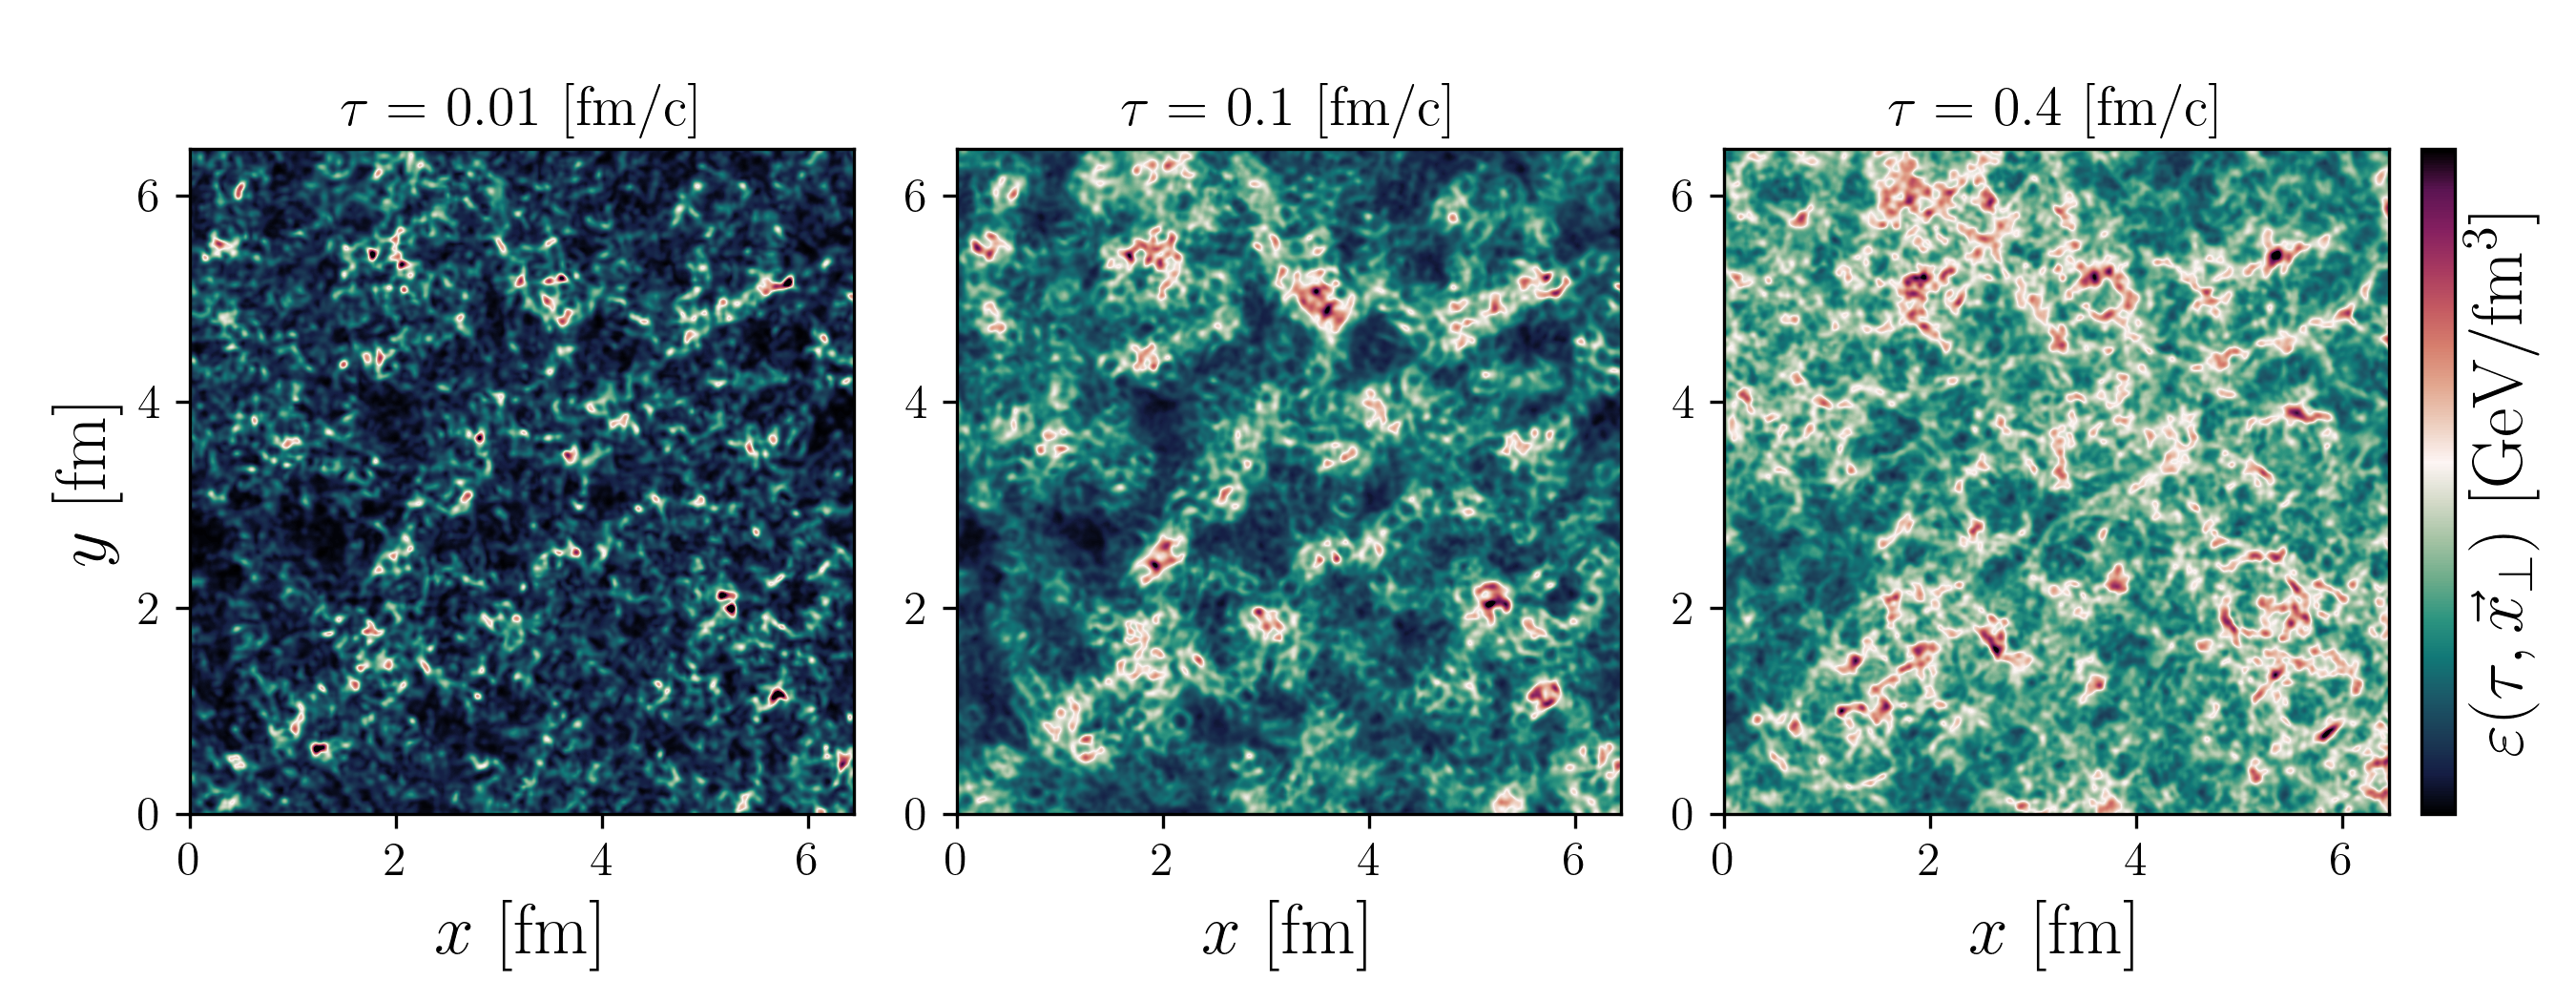
\includegraphics{flux_tubes_auau_200_nums_1_dpi_300.png}
	\caption{\normalsize Energy density in the transverse plane at various values of the proper time. Simulation parameters: $N_s=1$, $N_T=1024$ and $\Delta\tau=a_T/8$. In this plot, only a quarter of the simulation box is showed.}
\end{figure*}

\begin{figure}[!hbt]
	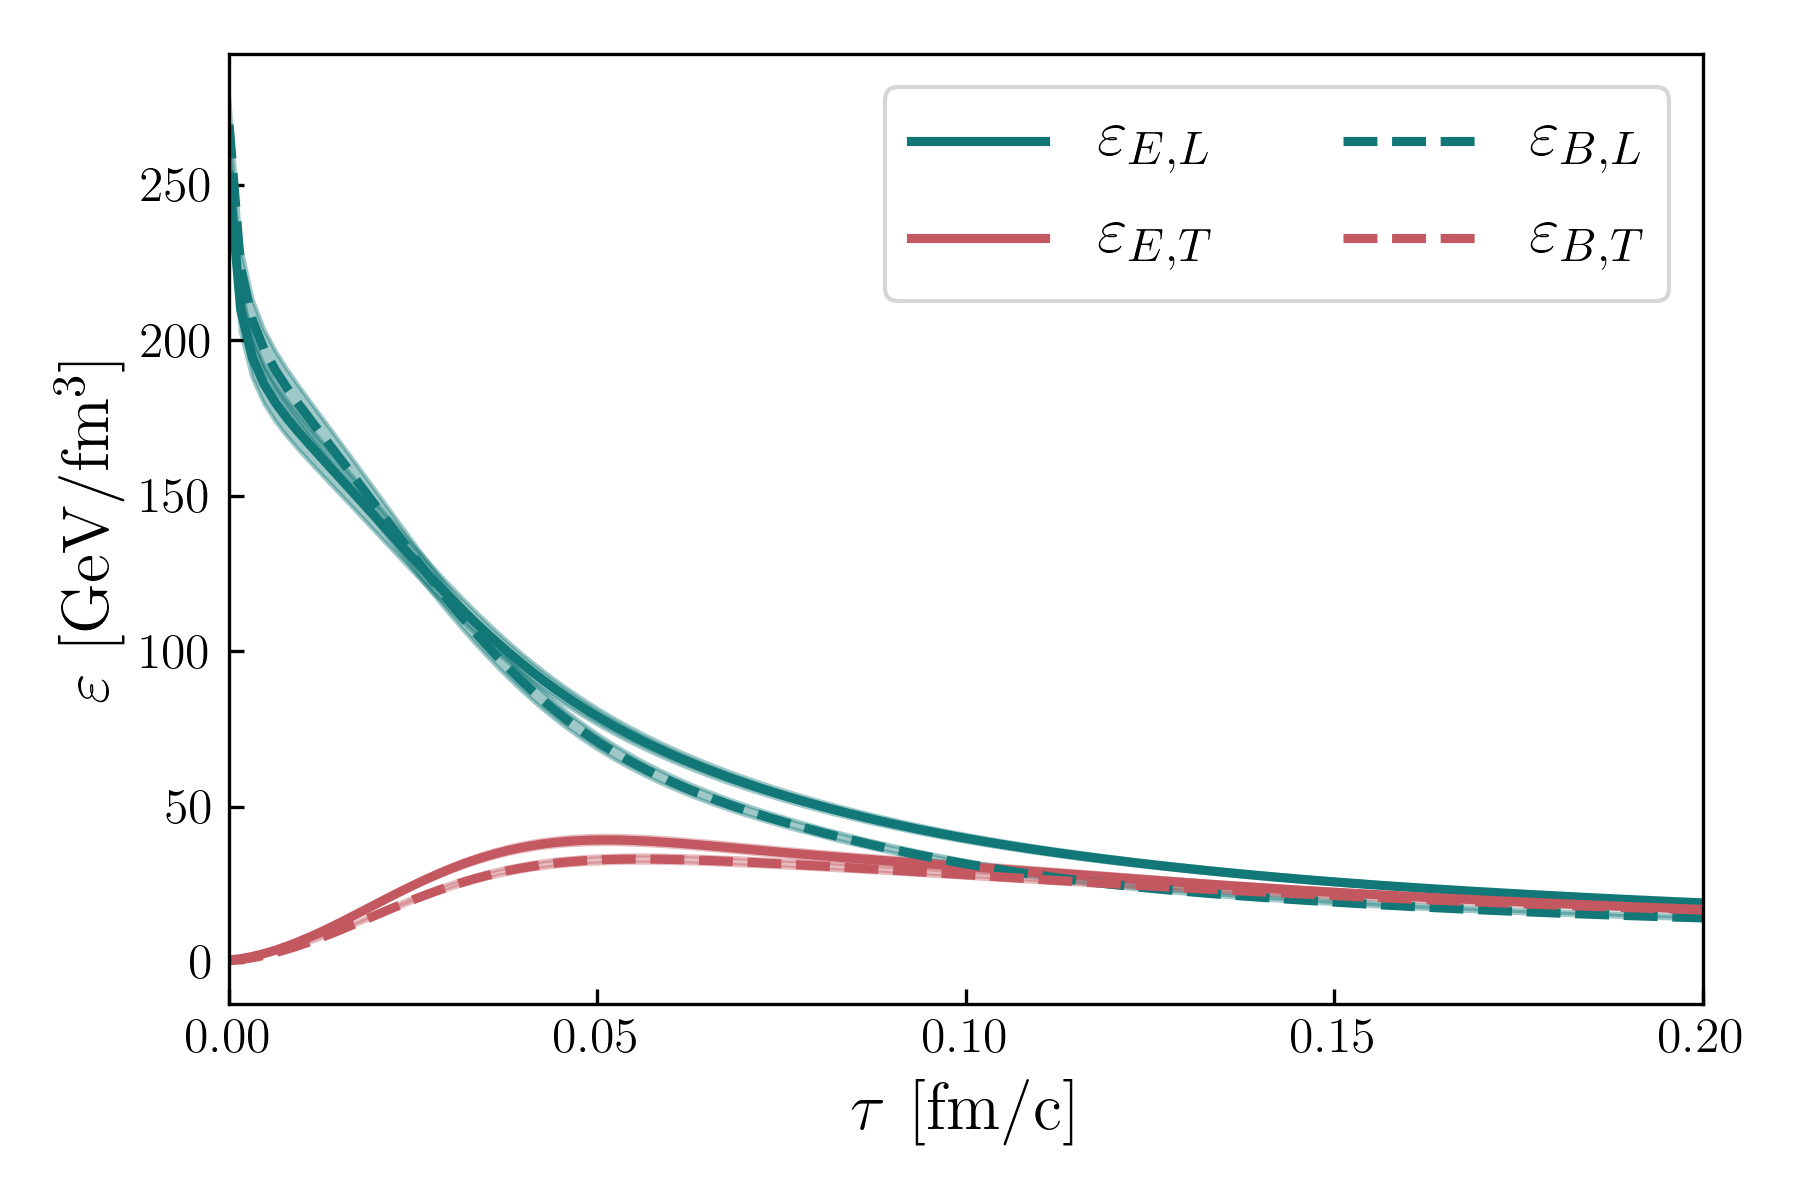
\includegraphics[width=\textwidth]{ed_components_auau_su3_200_dpi_300.png}
	\caption{\normalsize Longitudinal and transverse, electric and magnetic contributions to the energy density as a function of proper time, averaged over the transverse plane and over multiple events. Simulation parameters: $N_s=1$, $N_T=512$, $\Delta\tau=a_T/8$ and $N_\text{events}=30$. After $\tau\approx\textsf{Q}_s^{-1}$, all the components of the energy density become equal.}
\end{figure}

The picture that emerges is the following: initially,\sidenote{See the plot at $\tau=0.01$ fm/c.}the Glasma is mainly composed of longitudinal colored electric and magnetic fields, commonly referred to as {\sffamily\color{ming}flux tubes}. Once the Glasma evolves,\sidenote{At $\tau=0.1$ fm/c $\approx \textsf{Q}_s^{-1}$.}these flux tubes begin to expand in the transverse plane and circular patterns form. The longitudinal components of the energy density start to decrease while the transverse ones increase. This takes place until\sidenote{Look at the plot captured at $\tau=0.4$ fm/c.}all these components become equal and the system homogenizes. This description of the Glasma evolution may further be supported by looking at how the energy density and its components evolve with respect to the proper time. 

\begin{figure}[!hbt]
	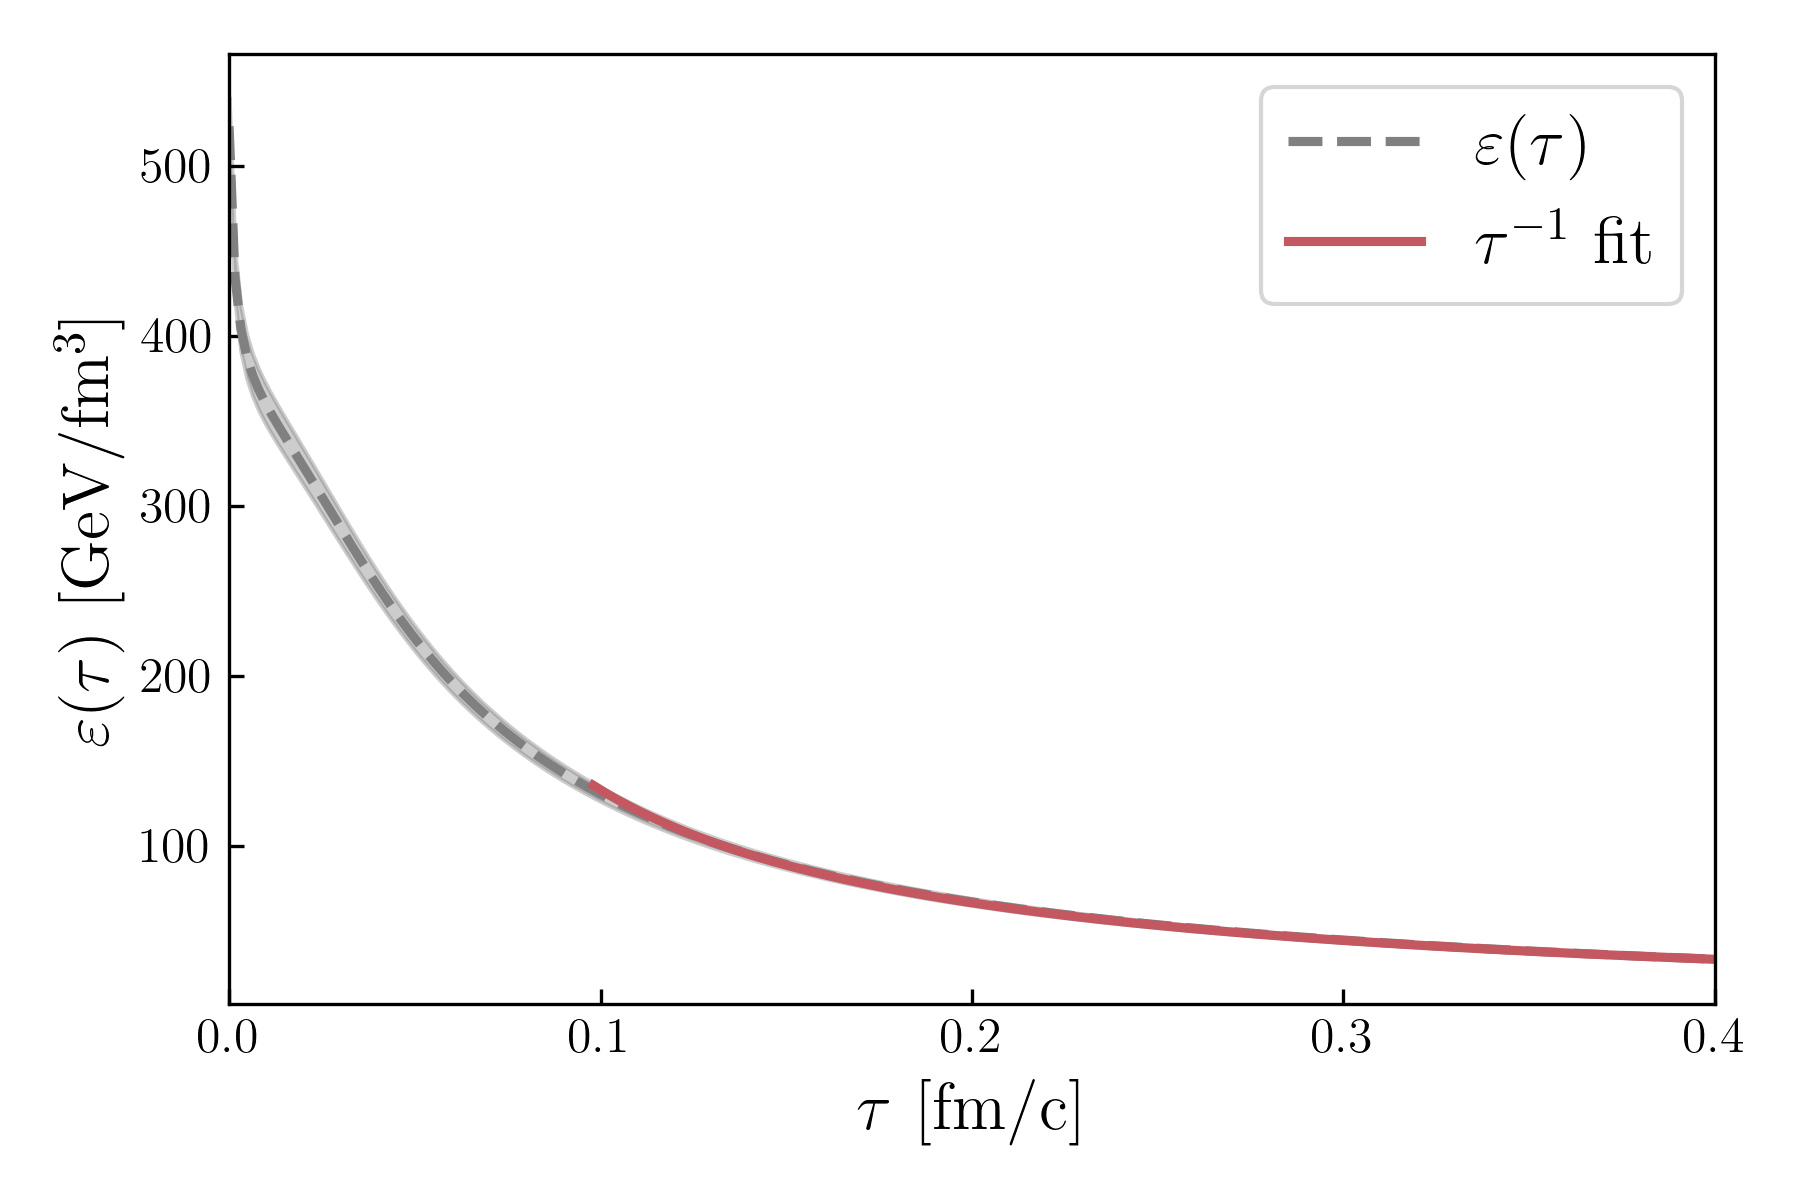
\includegraphics[width=\textwidth]{ed_auau_su3_200_dpi_300.png}
	\caption{\normalsize Energy density as a function of proper time, averaged over the transverse plane and over multiple events. Simulation parameters: $N_s=1$, $N_T=512$, $\Delta\tau=a_T/8$ and $N_\text{events}=30$. After $\tau\approx\textsf{Q}_s^{-1}$, the energy density becomes that of a Bjorken type boost-invariant expansion, namely $\tau\varepsilon(\tau)\approx \text{const.}$}
\end{figure}

One may extract $\varepsilon(\tau=0.01\text{ fm/c})\approx 134\text{ GeV/fm}^3$, which is comparable with the value $\varepsilon(\tau=0.01\text{ fm/c})\approx 130\text{ GeV/fm}^3$ obtained in \cite{lappiglasma}.

Qualitatively, the same results\sidenote{See the plots from \cite{muller} obtained with a previous version of {\sffamily Curraun} which may be found at \url{https://gitlab.com/dmueller/curraun_cy}.}may be obtained by using $\textsf{SU}(2)$ as a gauge group, instead of $\textsf{SU}(3)$, through scaling with an appropriate color factor.

\begin{figure}[!hbt]
	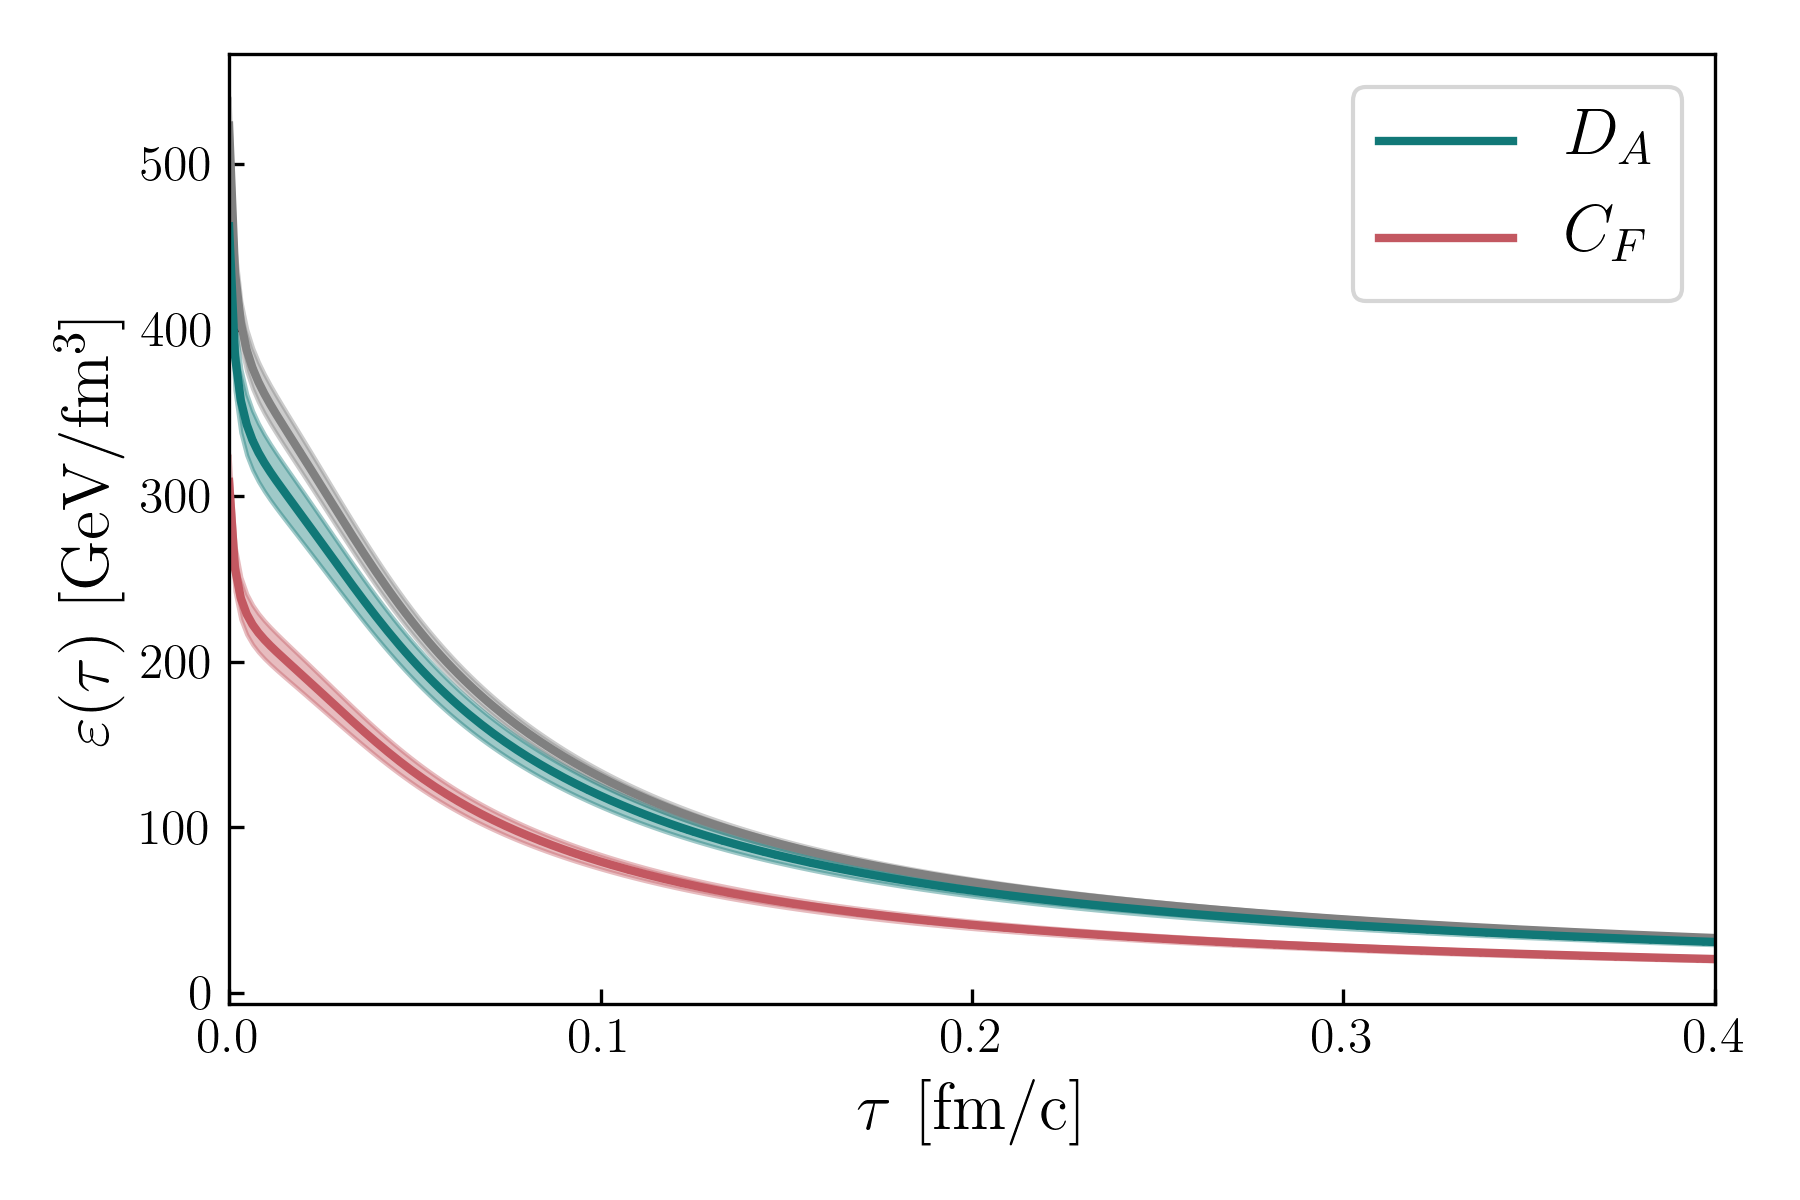
\includegraphics[width=\textwidth]{ed_comparison_auau_200_dpi_300.png}
	\caption{\normalsize Comparison between the energy density obtained using $\textsf{SU}(3)$ gauge group and $\textsf{SU}(2)$ respectively, but scaled with either the Casimir in the fundamental representation $C_F(3)/C_F(2)=16/9$, or with the dimension of the adjoint representation $D_A(3)/D_A(2)=8/3$ with $D_A(N_c)=N_c^2-1$.}
\end{figure}

One may also study the dependence of the energy density on some numerical parameters, namely $N_s$ and $m$. The continuum limit of the generalized {\sffamily MV} model\sidenote{Which is analytically taken as $N_s\rightarrow\infty$.}may numerically be chosen at $N_s=50$ since for values of $m\approx 0.2$ GeV and greater, increasing $N_s$ will not bring any significant differences.

\begin{figure}[!hbt]
	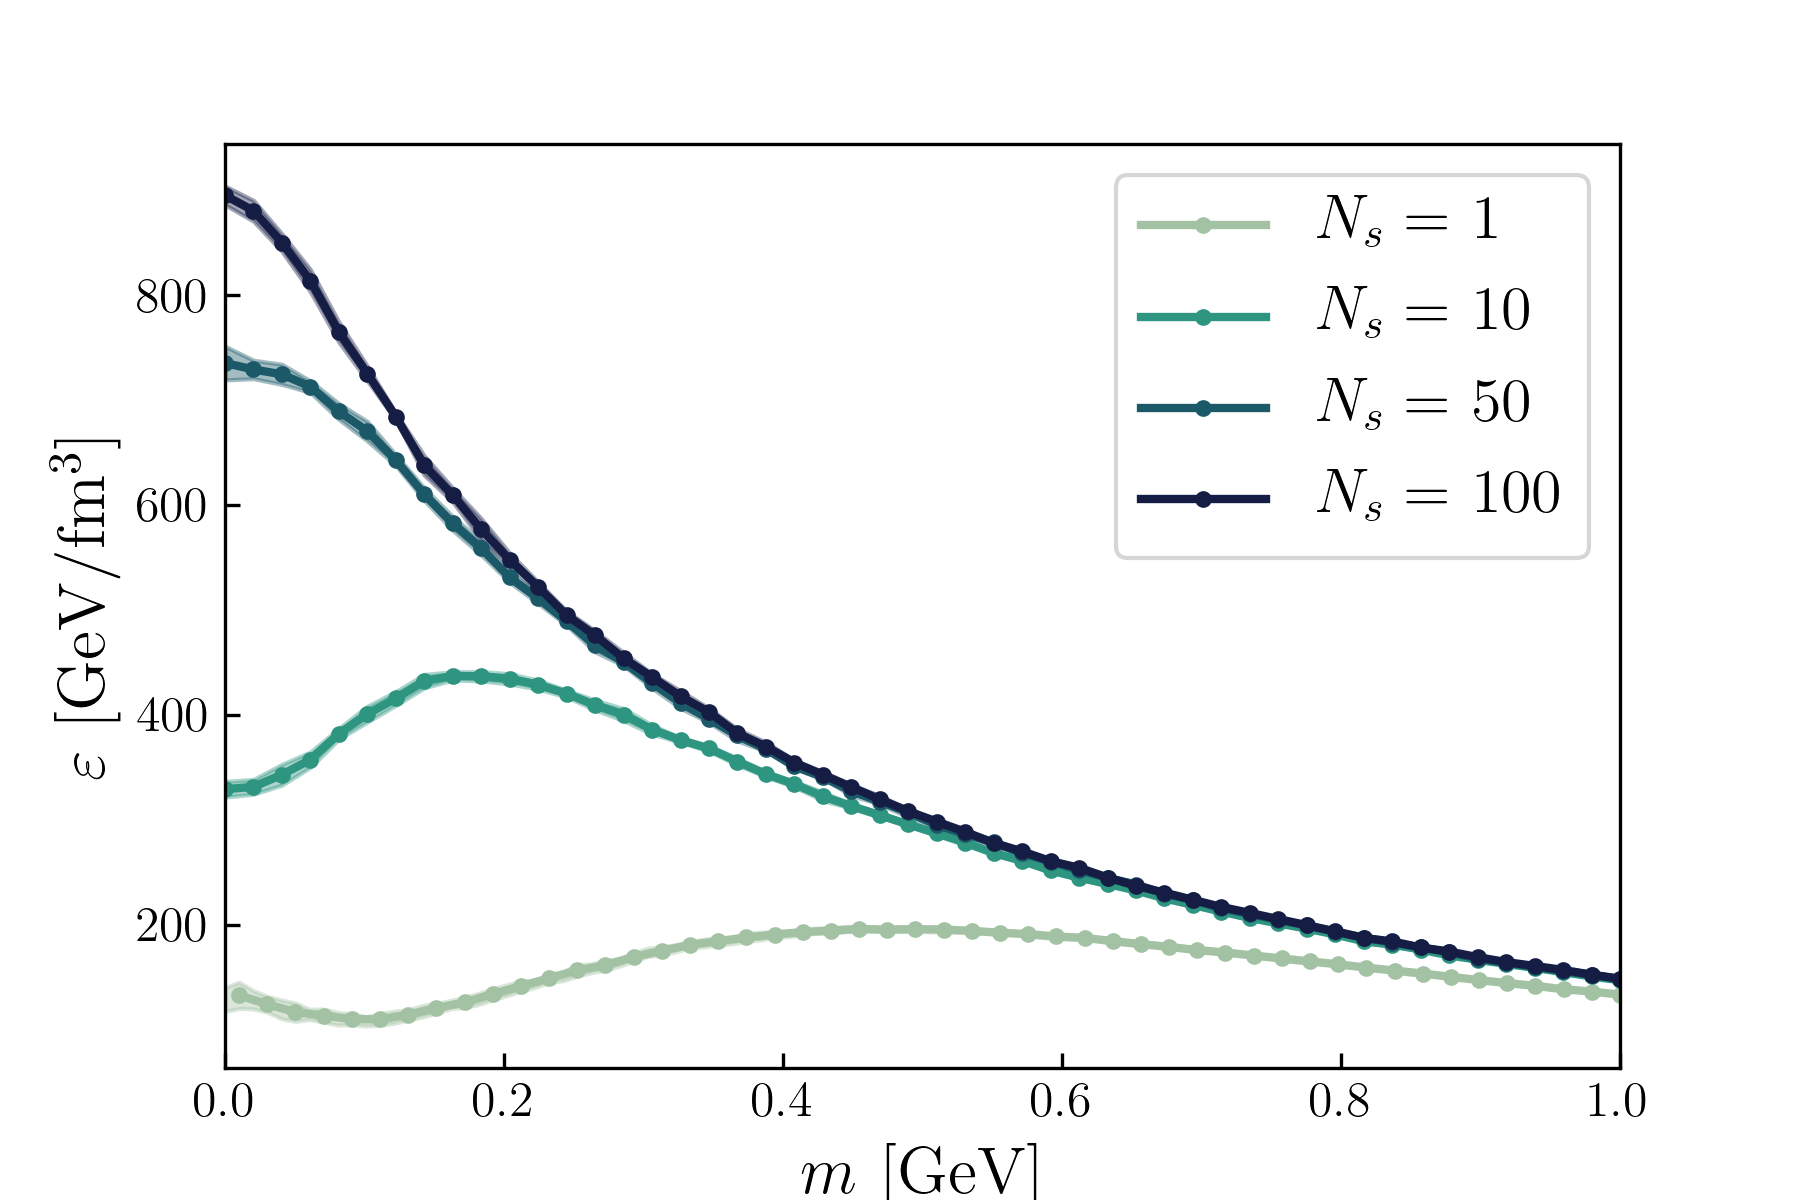
\includegraphics[width=\textwidth]{ed_sheets.png}
	\caption{\normalsize Energy density at $\tau=0.1$ fm/c as a function of $m$ for various values of $N_s$, averaged over multiple events. Simulation parameters: $N_T=512$, $\Delta\tau=a_T/8$ and $N_\text{events}=30$.} 
\end{figure}

The longitudinal and transverse pressure components reveal yet another peculiar aspect of the Glasma, namely {\sffamily\color{ming}pressure anisotropy}. The Yang-Mills fields of the Glasma generate pressures which satisfy\sidenote{As opposed to an isotropic system, for which the pressures should reach
\begin{align*}
    \lim\limits_{\tau\rightarrow\infty}p_L=\lim\limits_{\tau\rightarrow\infty}p_L=\frac{\varepsilon}{3}.
\end{align*}
}
\begin{equation*}
    \begin{aligned}
        \lim\limits_{\tau\rightarrow\infty}p_L=0, && \lim\limits_{\tau\rightarrow\infty}p_T=\frac{\varepsilon}{2}.
    \end{aligned}
\end{equation*}

\begin{figure}[!hbt]
	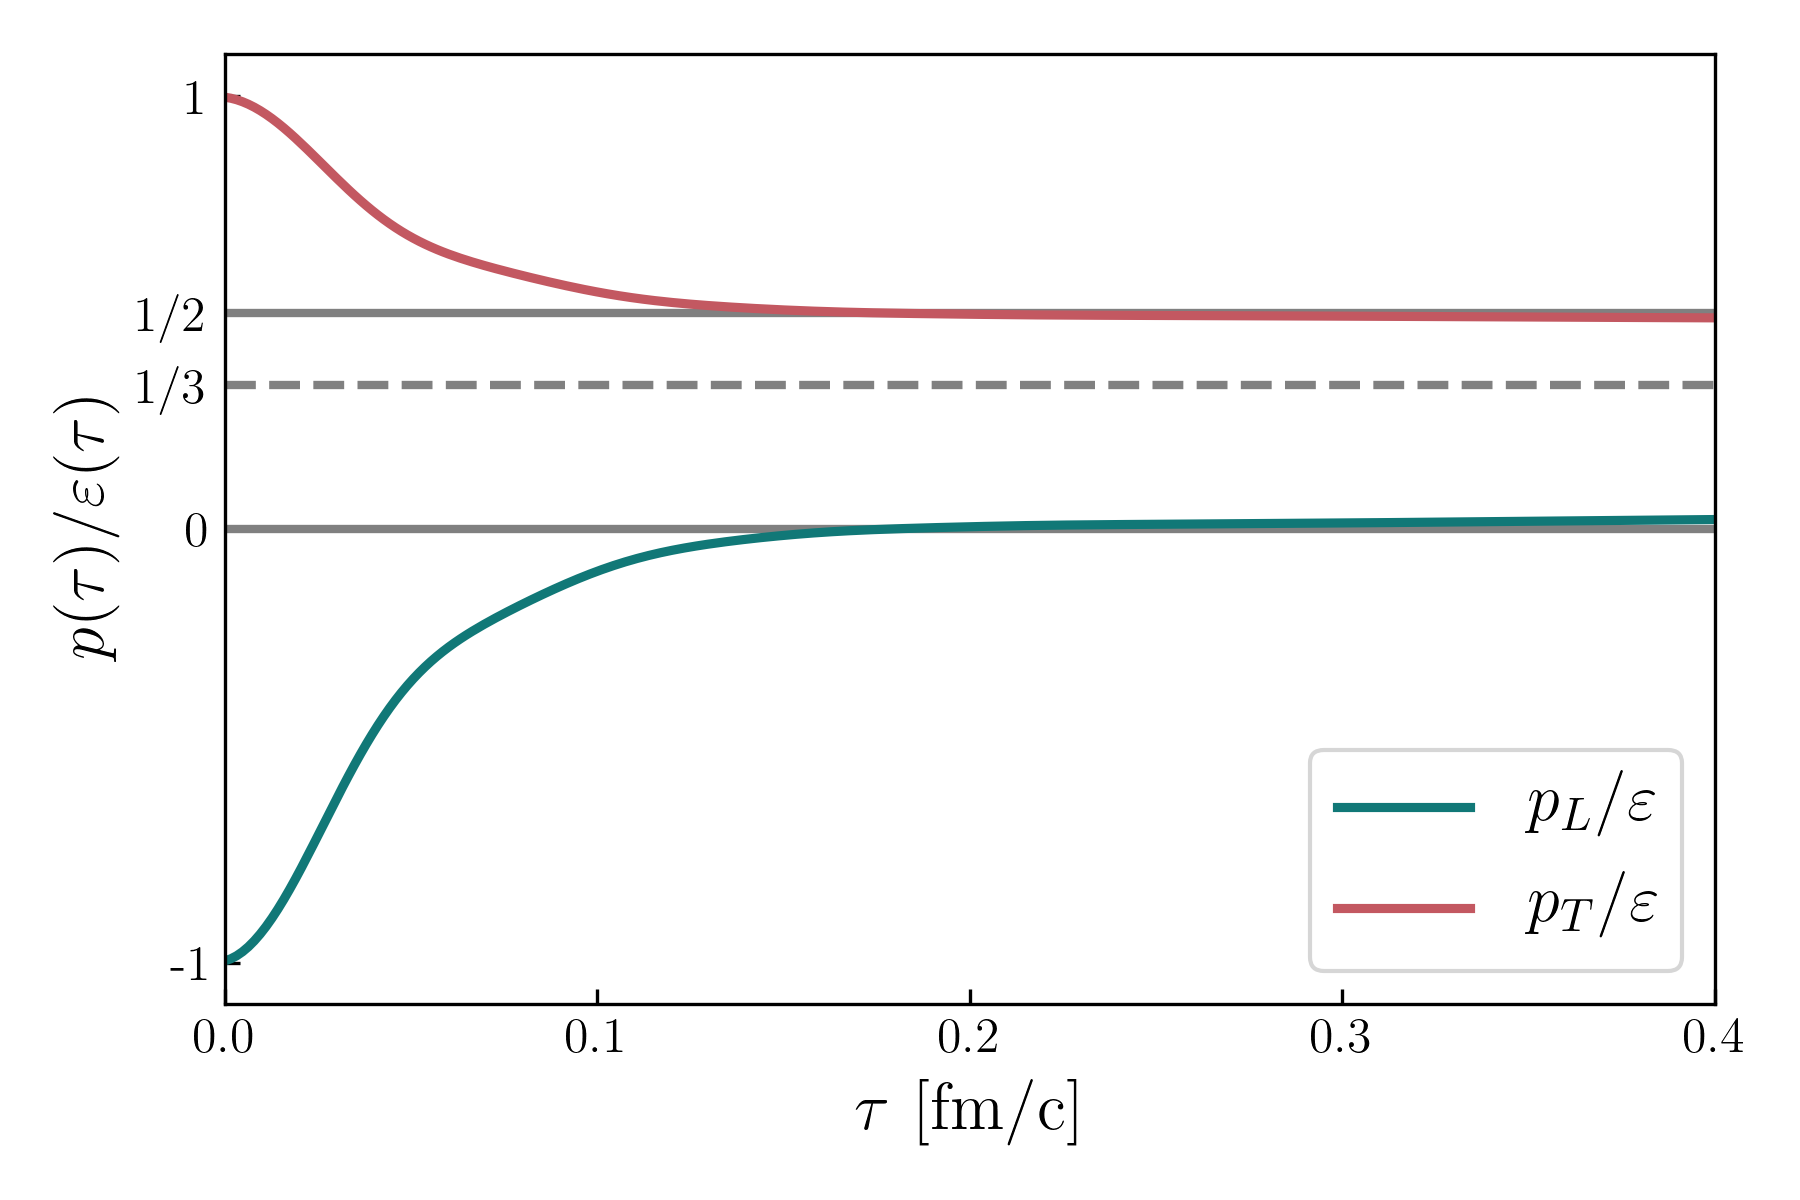
\includegraphics[width=\textwidth]{pressure_energy_ratio_su3_auau_200_dpi_300.png}
	\caption{\normalsize Longitudinal and transverse pressure to energy density ratio as a function of proper time, averaged over multiple events. Simulation parameters: $N_s=1$, $N_T=512$, $\Delta\tau=a_T/8$ and $N_\text{events}=30$. The Glasma never reaches pressure isotropy.} 
\end{figure}

This feature of the Glasma is problematic since it doesn't allow a smooth coupling to ideal or viscous hydrodynamics, in which the system is assumed to be at local equilibrium and isotropic. There exist various workarounds to surpass this problem: add quantum fluctuations on top of the classic field, which would then bring the system towards a state were hydrodynamics becomes applicable\sidenote{See \cite{epelbaum} for example.}; use an intermediate stage between the classic description of the Glasma and the hydrodynamic evolution of the QGP, based on an effective kinetic theory;\sidenote{Such an approach is described in \cite{kurkela1, kurkela2}.}apply anisotropic hydrodynamics,\sidenote{Reviews of this topic may be found at \cite{alqahtani, strickland}.}a modified version of relativistic hydrodynamics which accommodates large momentum anisotropies, as those generated in heavy-ion collisions.
 
%  \vspace{1cm}
% \begin{fullwidth}
% \begin{summary}[]
% [...]
% \end{summary}
% \end{fullwidth}

